\section{Protocol Layers}

The following is focused on the communication protocol in the \gls{CIoT}-Uu interface, it consist of six layers respectively:
\begin{itemize}
	\item \gls{NAS} layer
	\item \gls{RRC} layer
	\item \gls{PDCP} layer
	\item \gls{RLC} layer
	\item \gls{MAC} layer
	\item \gls{PHY} layer
\end{itemize}

The purpose and functionalities of these layers are explained in the following.

\subsection{NAS}
The \gls{NAS} layer is the top layer in the control plane. It signals directly between the \gls{UE} and the \gls{MME} \citep[ch. 3]{book_LTE_for_UMTS}. There are two protocols in the \gls{NAS} layer, the \gls{EMM} and the \gls{ESM}. The \gls{EMM} handles re-activation from idle mode. The \gls{UE} initiated case is called service request, the network initiated case is called paging. The \gls{EMM} protocol is used for handling attachment and detachment from the system when the \gls{UE} is in idle mode, in connected mode lower layer protocols handles this instead \citep[ch. 3]{book_LTE_for_UMTS}. It has been suggested that a new protocol should be implemented allowing the device to transmit a small amount of data directly in the \gls{NAS} layer, the details of this protocol has not yet been established \citep{REL-13}. 

\subsection{RRC} \label{sec:RRC}
The \gls{RRC} layer of the protocol is strictly control plane layer. It handles a great deal of control functions in the system including transition between device states and bearer request. The functionalities provided by the \gls{RRC} is \citep[ch. 6.6]{book_LTE_for_UMTS}:

\begin{itemize}
	\item Broadcast of system information
	\item Paging
	\item Establishment, maintenance and release of an \gls{RRC} connection between \gls{UE} and the \gls{eNB}
	\item Security functions including key management
	\item Establishment, maintenance and release of point to point radio bearers
	\item \gls{UE} measurement reporting and control of the reporting
	%\item Handover
	\item \gls{UE} cell selection and reselections and control of cell selection and reselection
	\item Context transfer between \gls{eNB}s
	\item \gls{UE} capability transfer
	\item Generic protocol error handling
	\item Support of self-configuration and self-optimization
\end{itemize}

One of the biggest changes from \gls{LTE} to \gls{NB-IoT} is the focus on reducing power consumption therefore a new state has been introduced compared to the \gls{LTE} system this can be seen in \autoref{fig:UE-states}.

\tikzsetnextfilename{state-diagram}
\begin{figure}[H]
\centering
\usetikzlibrary{arrows}
%\usetikzlibrary{shapes.multipart}
\renewcommand{\arraystretch}{0.8}
\resizebox{\textwidth}{!}{
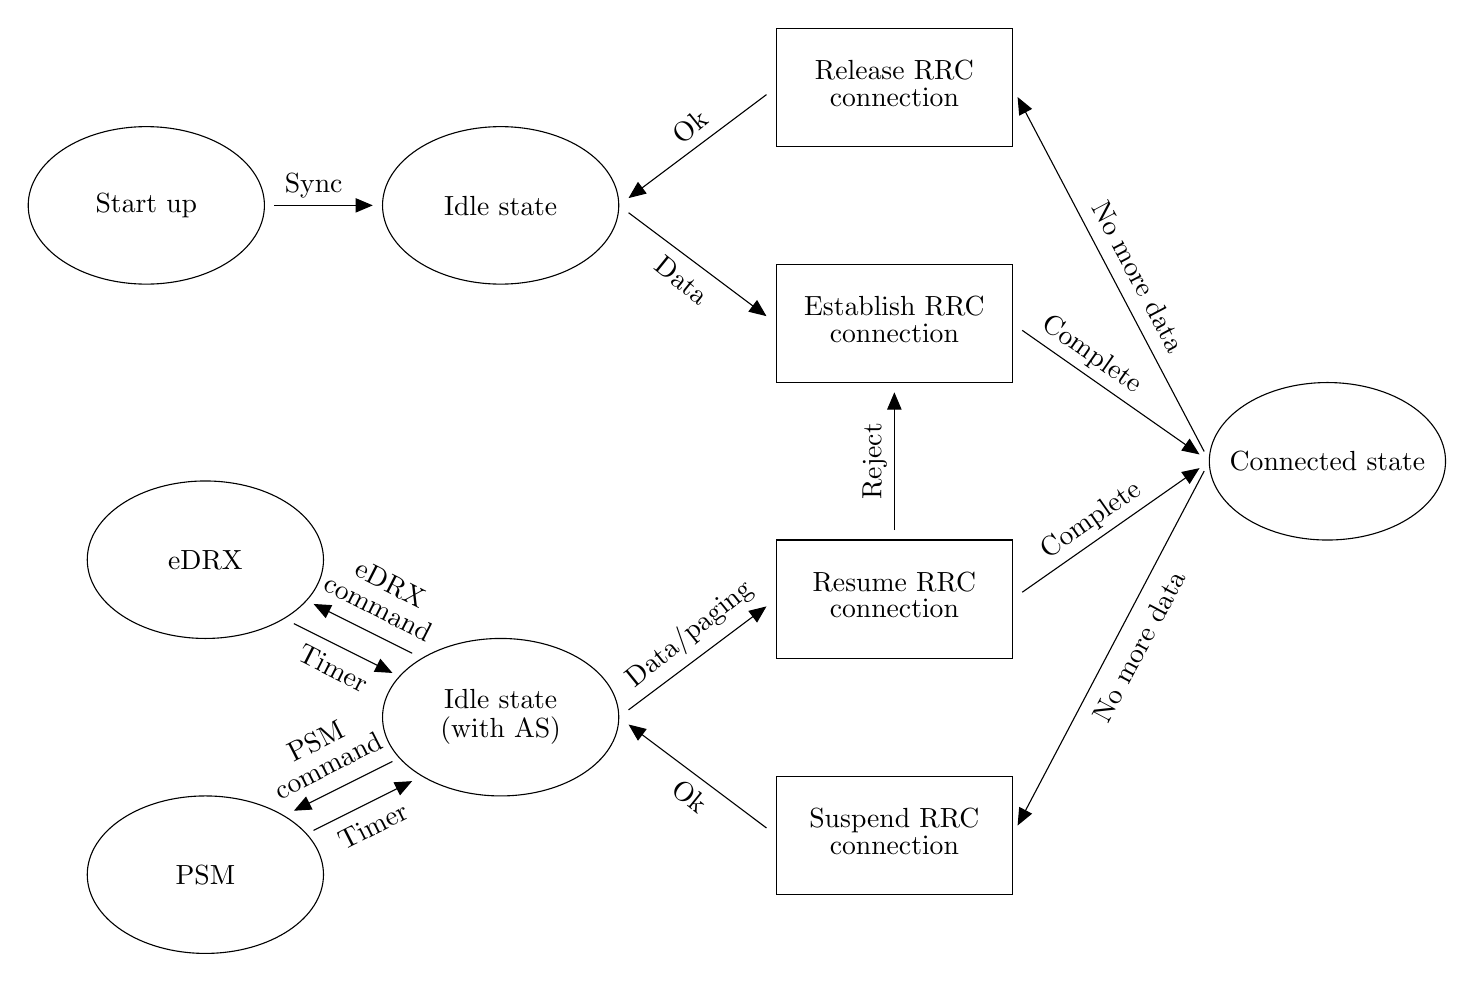
\begin{tikzpicture}[scale=0.5]

\draw  (-26,28) ellipse (3 and 2);
\node at (-26,28) {Start up};

\draw  (-17,28) ellipse (3 and 2);
\node at (-17,28) {Idle state};

\draw  (-24.5,11) ellipse (3 and 2);
%\node at (-17,15) {\acrshort{PSM}};
\node at (-24.5,11) {PSM};

\draw  (-10,19.5) rectangle (-4,16.5);
\node at (-7,18) {\begin{tabular}{c} Resume RRC \\ connection \end{tabular}};

\draw  (-10,26.5) rectangle (-4,23.5);
\node at (-7,25) {\begin{tabular}{c} Establish RRC \\ connection\end{tabular}};

\draw  (-10,13.5) rectangle (-4,10.5);
\node at (-7,12) {\begin{tabular}{c} Suspend RRC \\ connection\end{tabular}};

\draw  (-10,32.5) rectangle (-4,29.5);
\node at (-7,31) {\begin{tabular}{c} Release RRC \\ connection\end{tabular}};

\draw  (4,21.5) ellipse (3 and 2);
\node at (4,21.5) {Connected state};

\draw  (-17,15) ellipse (3 and 2);
\node at (-17,15) {\begin{tabular}{c} Idle state \\ (with AS)\end{tabular}};
\node (v22) at (-20,15) {};
\node (v23) at (-14,15) {};

\draw  (-24.5,19) ellipse (3 and 2);
\node at (-24.5,19) {eDRX};
\node (v25) at (-19,16.5) {};
\node (v26) at (-22,18) {};
\node (v27) at (-22.5,17.5) {};
\node (v28) at (-19.5,16) {};
\node[rotate=27] at (-21.5,14) {\begin{tabular}{c} PSM\\ command\end{tabular}};
\node[rotate=27] at (-20.25,12.25) {Timer};




\node (v1) at (-23,28) {};
\node (v2) at (-20,28) {};
\node (v3) at (-14,28) {};
\node (v4) at (-10,25) {};
\node (v5) at (-4,25) {};
\node (v6) at (1,21.5) {};
\node (v7) at (-4,12) {};
\node (v8) at (-4,31) {};
\node (v9) at (-4,18) {};
\node (v10) at (-10,18) {};
\node (v11) at (-10,12) {};
\node (v12) at (-10,31) {};
\node (v13) at (-7,19.5) {};
\node (v14) at (-7,23.5) {};
\node (v15) at (-19.5,14) {};
\node (v16) at (-22.5,12.5) {};
\node (v17) at (-22,12) {};
\node (v18) at (-19,13.5) {};



\draw [arrows={- triangle 45}] (v1) edge (v2);
\draw [arrows={- triangle 45}] (v23) edge (v10);
\draw [arrows={- triangle 45}] (v3) edge (v4);
%\draw [arrows={triangle 45-}]  (v4) edge ($(midpoint)+(0,0)$);

\draw [arrows={- triangle 45}] (v11) edge (v23);
\draw [arrows={- triangle 45}] (v12) edge (v3);
\draw [arrows={- triangle 45}] (v13) edge (v14);
\draw [arrows={- triangle 45}] (v9) edge (v6);
\draw [arrows={- triangle 45}] (v5) edge (v6);
\draw [arrows={- triangle 45}] (v6) edge (v7);
\draw [arrows={- triangle 45}] (v6) edge (v8);
\draw [arrows={- triangle 45}] (v15) edge (v16);
\draw [arrows={- triangle 45}]  (v17) edge (v18);
\draw [arrows={- triangle 45}] (v25) edge (v26);
\draw [arrows={- triangle 45}]  (v27) edge (v28);


\node at (-21.75,28.5) {Sync};
\node[rotate=-27] at (-20,18) {\begin{tabular}{c} eDRX \\ command\end{tabular}};
\node[rotate=-27] at (-21.25,16.25) {Timer};
\node[rotate=39] at (-12.2,30) {Ok};
\node[rotate=39] at (-12.2,17.1) {Data/paging};
\node[rotate=-39] at (-12.2,13) {Ok};
\node[rotate=-39] at (-12.4,26.1) {Data};
\node[rotate=-35] at (-2,24.2) {Complete};
\node[rotate=35] at (-2,20) {Complete};
\node[rotate=62] at (-0.8,16.8) {No more data};
\node[rotate=-62] at (-0.8,26.2) {No more data};
\node[rotate=90] at (-7.5,21.5) {Reject};


\end{tikzpicture}
}
\caption{State diagram with transition options for a \gls{UE}.}
\label{fig:UE-states}
\end{figure}


With this new structure comes a greater focus on \gls{RRC} resume connection, which is very advantageous with regards to power consumption as it allows the device to suspend its connection and save its \gls{AS} go into \gls{eDRX}, when it then wakes up again it can make a resume request where it uses its previous \gls{AS} to transmit its data reducing the overhead considerably. This can also be seen from \autoref{tab:signaling_comparison} where a comparison between the different procedures is shown. 

\begin{table}[H]
\centering
\resizebox{\textwidth}{!}{
\begin{tabular}{|p{2.5cm}|p{4cm}|p{4cm}|p{4cm}|} \hline
\rowcolor{gray!50}\textbf{Direction} & \raggedright\arraybackslash\textbf{Legacy Service Request Procedure}	& \raggedright\arraybackslash\textbf{\gls{RRC} Connection Resume} & \textbf{Control Plane Data Transfer}  \\\hline
UL	& \multicolumn{3}{c|}{Preamble} \\\hline
\rowcolor{gray!10}DL	& \multicolumn{3}{c|}{\gls{RAR}} \\\hline
UL	& \raggedright\arraybackslash \gls{RRC} Connection Request						& \raggedright\arraybackslash \gls{RRC} Connection Resume Request	& \raggedright\arraybackslash \gls{RRC} Connection Request \\\hline
\rowcolor{gray!10}DL	& \raggedright\arraybackslash \gls{RRC} Connection Setup						& \raggedright\arraybackslash \gls{RRC} Connection Resume 			& \raggedright\arraybackslash \gls{RRC} Connection Setup   \\\hline
UL	& \raggedright\arraybackslash \gls{RRC} Connection Request Complete 			& \raggedright\arraybackslash \gls{RRC} Connection Resume Complete & \raggedright\arraybackslash \gls{RRC} Connection Complete  \\\hline
\rowcolor{gray!10}DL	& \raggedright\arraybackslash Security Mode Command 							& - & -  \\\hline
UL	& \raggedright\arraybackslash Security Mode Complete 							& - & -  \\\hline
\rowcolor{gray!10}DL	& \raggedright\arraybackslash \gls{RRC} Connection Reconfiguration 			& - & -  \\\hline
UL	& \raggedright\arraybackslash \gls{RRC} Connection Reconfiguration Complete 	& - & -  \\\hline
\raggedright\arraybackslash \textbf{Total number of messages} 					& \textbf{9} & \textbf{5} & \textbf{5} \\\hline
\end{tabular}
}
\caption{Signaling comparison between different methods \citep{REL-13}}
\label{tab:signaling_comparison}
\end{table}

\textbf{\Gls{SRB}}\\
The \gls{RRC} sets up three different \gls{SRB}s. The \gls{SRB}s is used to carry \gls{RRC} and \gls{NAS} messages. \gls{SRB}0 is used for \gls{CCCH} during \gls{RRC} connection setup or during link failure, messages carried here include \gls{RRC} connection request, \gls{RRC} connection setup, \gls{RRC} connection reject, \gls{RRC} connection reestablishment request, \gls{RRC} connection reestablishment and \gls{RRC} connection reestablishment reject. \gls{SRB}1 is used when a \gls{RRC} connection is established, it is used to transfer both \gls{RRC} messages using \gls{DCCH} and \gls{NAS} messages until security is established. Once security is established the \gls{NAS} messages is carried on \gls{SRB}2 which has a lower priority. \citep[ch. 6.6]{book_LTE_for_UMTS} 


\textbf{\gls{SIB}s}\\
Before the device attempts to access the system it needs a lot of information about the system, that is carried in the \gls{SIB}s. For \gls{NB-IoT} there are eight different \gls{SIB}s messages. A list of the information carried in the different \gls{SIB}s can be seen in \autoref{tab:NB-SIB}. The \gls{RRC} takes care of updating these messages and paging the devices if changes occur.

\begin{table}[H]
\centering
\begin{tabular}{|p{3cm}|p{8cm}|p{3cm}|}\hline
\textbf{Name}		& \textbf{Information}																	& \textbf{Update rate}	\\\hline
\raggedright\arraybackslash\gls{MIB-NB}		& Essential information required to receive further system information 					& 640 ms				\\\hline
\raggedright\arraybackslash\gls{NB-SIB}1		& Cell access and selection, other SIB scheduling 										& 40.96 s 				\\\hline
\gls{NB-SIB}2		& Radio resource configuration information 												& NA 					\\\hline
\gls{NB-SIB}3		& Cell re-selection information for intra-frequency, inter-frequency 					& NA 					\\\hline
\gls{NB-SIB}4		& Neighboring cell related information relevant for intra-frequency cell re-selection 	& NA 					\\\hline
\gls{NB-SIB}5		& Neighboring cell related information relevant for inter-frequency cell re-selection 	& NA 					\\\hline
\gls{NB-SIB}14		& Access Barring parameters 															& Fast 					\\\hline
\gls{NB-SIB}16		& Information related to GPS time and Coordinated Universal Time (UTC) 					& Fast 					\\\hline
\end{tabular}
\caption{List of different \gls{SIB} messages and the information carried within \citep{whitepaper,REL-13}.}
\label{tab:NB-SIB}
\end{table}

\textbf{Paging} \\
Paging serves two main functions, the first is to notify a device in \gls{RRC} idle state to set up a \gls{RRC} connection to handle incoming data, the second is to inform the devices both in \gls{RRC} idle and \gls{RRC} connected state the system information has changed. \citep[ch. 7]{NB-IoT_Book}

\textbf{Establishment, Maintenance and Release of \gls{RRC} Connection} \\
When an \gls{RRC} connection setup is requested, the \gls{eNB} has the option to reject it with a wait timer if the network is overloaded and can set the access barrer parameters appropriately in the \gls{NB-SIB}14. In the \gls{RRC} connection request message the device can trasmit its \gls{S-TMSI} if it possess a valid version else it will transmit a 40 bits random value. Five different establishment causes has been defined: emergency, high-priority access, mobility-terminated access, mobile-originated signaling and mobile-originated data. In \gls{NB-SIB}1 there exists at most six different \gls{PLMN} identities, the device selects one and reports it in the  \gls{RRC} connection setup complete message along with any \gls{MME} the device might already be registered to. The \gls{eNB} then finds the \gls{MME} and starts the S1 connection setup. When a connection setup is successful the device moves to the \gls{RRC} connected state. \citep[ch. 6.6]{book_LTE_for_UMTS}

%\todo{should we put detailed connection options in here, should we go in detail with further RRC functions and what about radio bearers}

%\textbf{\gls{UE} Measurement Reporting and Control of the Reporting} \\


%%% pic for rrc connection resume
%\begin{figure}[H]
%\centering
%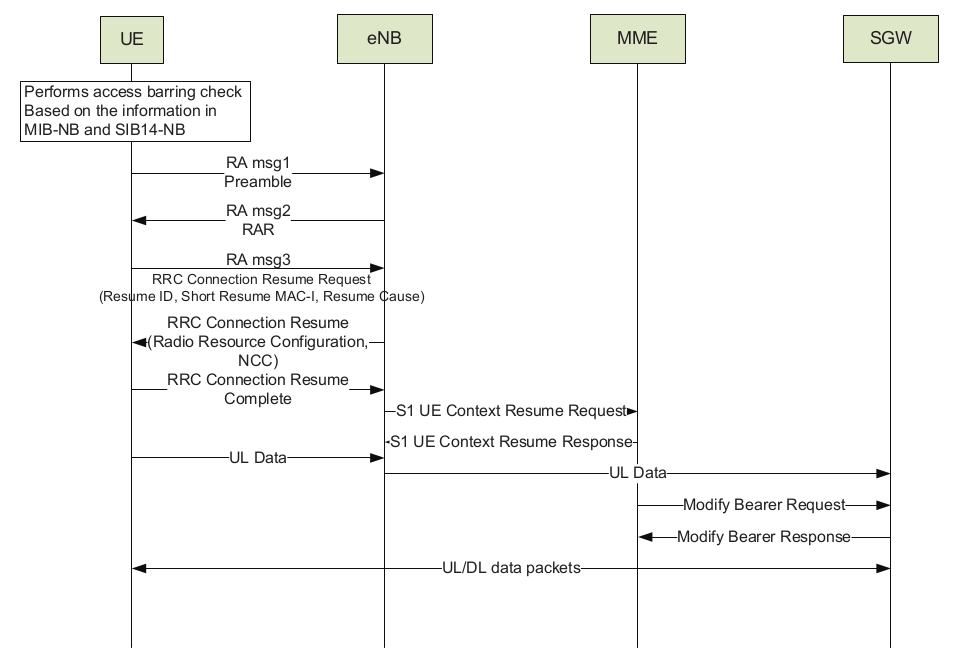
\includegraphics[width=\textwidth]{figures/RRC_resume.png}
%\caption{Signaling procedure for a \gls{RRC} resume request}
%\label{fig:RRC_resume}
%\end{figure}

\subsection{PDCP}
The \gls{PDCP} layer is just below the \gls{RRC} it handles both control functions as well as user data. The key function of the \gls{PDCP} include \citep[ch. 6.5]{book_LTE_for_UMTS}:
\begin{itemize}
	\item Header compression and decompression of \gls{IP} packets. This is an important function especially for small data packets as the overhead could become quite significant.
	\item Ciphering and deciphering of both user plane and most of control plane data.
	\item Integrity protection and verification to ensure control data comes from the correct source.
\end{itemize}

The \gls{PDCP} gets \gls{PDCP} \gls{SDU}s from the \gls{RRC} and \gls{NAS} layer. 

\tikzsetnextfilename{PDCP_data_flow}
\begin{figure}[H]
\centering
\resizebox{0.8\textwidth}{!}{
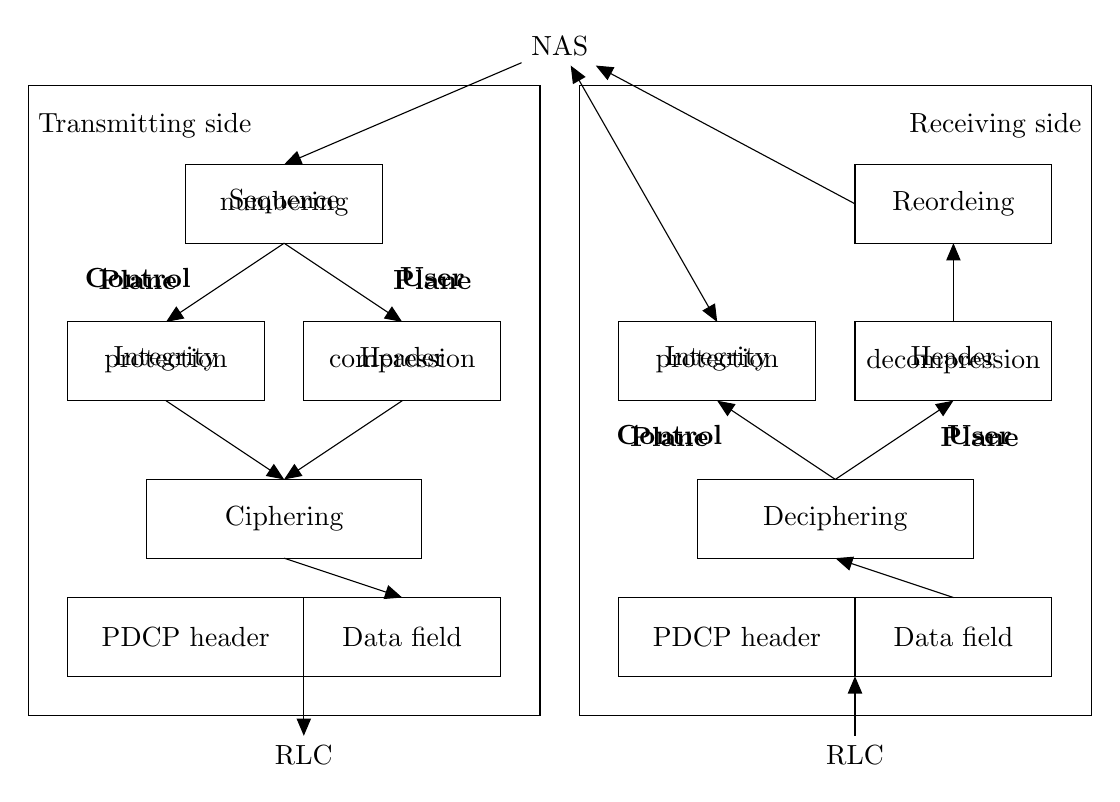
\begin{tikzpicture}[scale=.5]


\node (v2) at (-0.5,8) {NAS};
\draw  (-1,7) rectangle (-14,-9);
\draw  (0,7) rectangle (13,-9);
\node[anchor=west] at (-14,6) {Transmitting side};
\node[anchor=east] at (13,6) {Receiving side};

\draw  (-10,5) rectangle (-5,3);
\node at (-7.5,4) {\begin{tabular}{c} Sequence \\[-0.9em] numbering \end{tabular}};
\draw  (-13,1) rectangle (-8,-1);
\node at (-10.5,0) {\begin{tabular}{c} Integrity \\[-0.9em] protection \end{tabular}};
\draw  (-7,1) rectangle (-2,-1);
\node at (-4.5,0) {\begin{tabular}{c} Header \\[-0.9em] compression \end{tabular}};
\draw  (-11,-3) rectangle (-4,-5);
\node at (-7.5,-4) {Ciphering};
\draw  (-13,-6) rectangle (-7,-8) node (v1) {};
\draw  (v1) rectangle (-2,-6);
\node at (-10,-7) {PDCP header};
\node at (-4.5,-7) {Data field};
\node (v12) at (-7,-10) {RLC};

\node (v3) at (-7.5,5) {};
\node (v4) at (-7.5,3) {};
\node (v5) at (-10.5,1) {};
\node (v6) at (-4.5,1) {};
\node (v9) at (-4.5,-1) {};
\node (v7) at (-10.5,-1) {};
\node (v8) at (-7.5,-3) {};
\node (v10) at (-7,-5) {};
\node (v11) at (-4.5,-6) {};
\draw  [- triangle 45] (v2) -- (-7.5,5);
\draw  [- triangle 45] (-7.5,3) -- (-10.5,1);
\draw  [- triangle 45] (-7.5,3) -- (-4.5,1);
\draw  [- triangle 45] (-10.5,-1) -- (-7.5,-3);
\draw  [- triangle 45] (-4.5,-1) -- (-7.5,-3);
\draw  [- triangle 45] (-7.5,-5) -- (-4.5,-6);
\draw  [- triangle 45] (-7,-8) -- (v12);
\node[anchor=east] at (-9.2,2) {\begin{tabular}{c} \textbf{Control} \\[-0.9em] \textbf{Plane} \end{tabular}};
\node[anchor=west] at (-5.4,2) {\begin{tabular}{c} \textbf{User} \\[-0.9em] \textbf{Plane} \end{tabular}};

\draw  (12,5) rectangle (7,3);
\node at (9.5,4) {Reordeing};
\draw  (6,1) rectangle (1,-1);
\node at (3.5,0) {\begin{tabular}{c} Integrity \\[-0.9em] protection \end{tabular}};
\draw  (12,1) rectangle (7,-1);
\node at (9.5,0) {\begin{tabular}{c} Header \\[-0.9em] decompression \end{tabular}};
\draw  (10,-3) rectangle (3,-5);
\node at (6.5,-4) {Deciphering};
\draw  (12,-6) rectangle (7,-8) node (v1) {};
\draw  (v1) rectangle (1,-6);
\node at (4,-7) {PDCP header};
\node at (9.5,-7) {Data field};

\node (v3) at (-7.5,5) {};
\node (v4) at (-7.5,3) {};
\node (v5) at (3.5,1) {};
\node (v6) at (9.5,1) {};
\node (v9) at (9.5,-1) {};
\node (v7) at (3.5,-1) {};
\node (v8) at (6.5,-3) {};
\node (v10) at (6,-5) {};
\node (v11) at (9.5,-6) {};
\node (v14) at (9.5,3) {};
\node (v15) at (7,4) {};
\node (v13) at (7,-10) {RLC};

\draw [- triangle 45] (v13) -- (7,-8);
\draw [- triangle 45] (9.5,-6) -- (6.5,-5);
\draw [- triangle 45] (6.5,-3) -- (3.5,-1);
\draw [- triangle 45] (6.5,-3) -- (9.5,-1);
\draw [- triangle 45] (9.5,1) -- (9.5,3);
\draw [- triangle 45] (7,4) -- (v2);
\draw [arrows={triangle 45 - triangle 45}] (3.5,1) -- (v2);
\node[anchor=east] at (4.3,-2) {\begin{tabular}{c} \textbf{Control} \\[-0.9em] \textbf{Plane} \end{tabular}};
\node[anchor=west] at (8.5,-2) {\begin{tabular}{c} \textbf{User} \\[-0.9em] \textbf{Plane} \end{tabular}};

\end{tikzpicture}}
\caption{\gls{PDCP} layer operation with associated \gls{PDCP} \gls{SDU} \citep[fig. 6.12]{book_LTE_for_UMTS}}
\label{fig:PDCP_operation}
\end{figure}

As can be seen in \autoref{fig:PDCP_operation} before forwarding the data to the \gls{RLC} layer, it is first numbered and then either integrity protection or header compression is applied, depending on whether or not it is control plane data or user plane data. It is then ciphered and forwarded. When the \gls{PDCP} receive data from the \gls{RLC} layer, it is first deciphered and again depending on whether it is control pane data or user plane data it is integrity protected or header decompression and reordered and then forwarded to the \gls{NAS}. \citep[ch. 6.5]{book_LTE_for_UMTS}  

%The \gls{PDCP} layer also handles alot during handovers, however as handovers is out of the scope for \gls{NB-IoT} these functionalities are obsolete. 

\subsection{RLC}

The \gls{RLC} layer has three basic functionalities \cite[ch. 6.4]{book_LTE_for_UMTS}

\begin{itemize}
	\item To transfer \gls{PDU}s from higher layers i.e. \gls{RRC}, \gls{NAS} or \gls{PDCP}
	\item Depending on the \gls{RLC} mode used, error correction with \gls{ARQ}, concatenation/segmentation, in-sequence delivery and duplicate detection may occur
	\item Protocol error handling to detect and recover from protocol error states caused by for example signaling errors
\end{itemize}

The modes mentioned before include \gls{TM}, \gls{UM} and \gls{AM} \citep[ch. 6.4]{book_LTE_for_UMTS}.

\textbf{\gls{TM} operation} \\
In \gls{TM} the \gls{RLC} receives and deliver the \gls{PDU}s without adding any header to it. Therefore it does not track received \gls{PDU}s between receiving and transmitting entities. This mode is only suitable for communication that does not require physical layer retransmission or the data is not sensitive to delivery order and is therefore not very suitable to \gls{NB-IoT}. 

\textbf{\gls{UM} operation} \\
The \gls{UM} adds some control functions to the data stream. It enables segmentation of the data and keeps track of sequence numbering. This mode also makes in-sequence delivery of out-of-sequence data, which can occur because of lower layer \gls{HARQ} operation. The data is segmented and a header is added which includes a sequence number to facilitate reordering and duplicate detection on the receiving side.

\textbf{\gls{AM} operation} \\
The \gls{AM} adds all the functionalities of the \gls{UM} but also provide retransmission, the header will in this case contain the last correctly received packet on the receiving side additionally to the sequence number. 

\captionsetup{belowskip=0em}
\begin{minipage}[H]{0.48\textwidth}
\tikzsetnextfilename{RLC_UM-SAP}
\begin{figure}[H]
\centering
\resizebox{\textwidth}{!}{
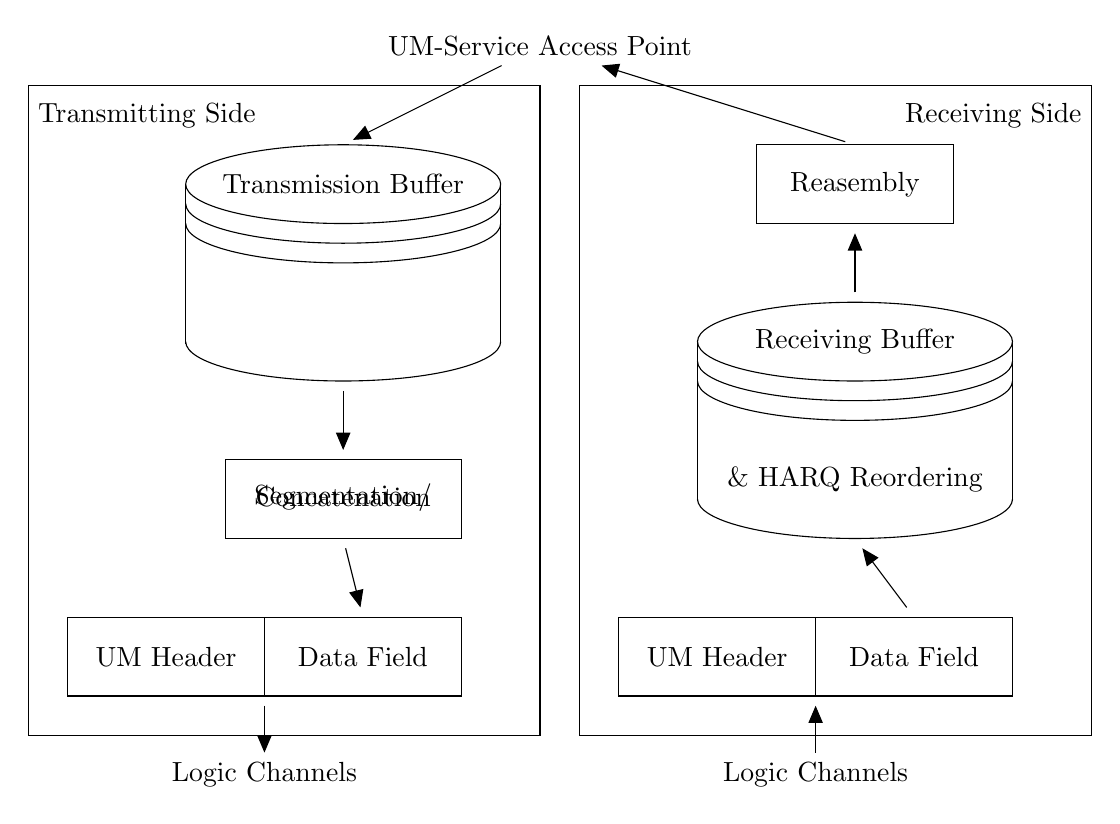
\begin{tikzpicture}[scale=.5]

\draw  (-1,8.5) rectangle (-14,-8);
\draw  (0,8.5) rectangle (13,-8);

\node (v1) at (-6,6) {Transmission Buffer};
\draw  (v1) ellipse (4 and 1);
\draw (-10,5.5) arc (180:360:4 and 1);
\draw (-10,5) arc (180:360:4 and 1);
\draw (-10,2) arc (180:360:4 and 1);
\node (v2) at (-10,6) {};
\node (v4) at (-2,6) {};
\node (v3) at (-10,1.7) {};
\node (v5) at (-2,1.7) {};
\draw  (v2) ++(0,0) edge (v3);
\draw  (v4)  ++(0,0) edge (v5);

\draw  (-9,-1) rectangle (-3,-3);
\node at (-6,-2) {\begin{tabular}{c} Segmentation/ \\[-0.9em] Concatenation\end{tabular}};
\draw  (-13,-5) rectangle (-8,-7) node (v6) {};
\draw  (v6) rectangle (-3,-5);
\node at (-10.5,-6) {UM Header};
\node at (-5.5,-6) {Data Field};



\node (v10) at (7,2) {Receiving Buffer};
\draw  (v10) ellipse (4 and 1);
\draw (3,1.5) arc (180:360:4 and 1);
\draw (3,1) arc (180:360:4 and 1);
\draw (3,-2) arc (180:360:4 and 1);
\node (v20) at (3,2) {};
\node (v40) at (11,2) {};
\node (v30) at (3,-2.3) {};
\node (v50) at (11,-2.3) {};
\draw  (v20) ++(0,0) edge (v30);
\draw  (v40)  ++(0,0) edge (v50);


\draw  (4.5,7) rectangle (9.5,5);
\draw  (1,-5) rectangle (6,-7) node (v7) {};
\draw  (v7) rectangle (11,-5);
\node at (7,6) {Reasembly};
\node at (7,-1.5) {\& HARQ Reordering};
\node at (3.5,-6) {UM Header};
\node at (8.5,-6) {Data Field};

\node (v15) at (-8,-9) {Logic Channels};
\node (v16) at (6,-9) {Logic Channels};
\node (v14) at (-5.5,-5) {};
\node (v13) at (-6,-3) {};
\node (v11) at (-6,1) {};
\node (v9) at (-6,7) {};
\node (v8) at (-1,9.5) {UM-Service Access Point};
\node (v22) at (7,7) {};
\node (v21) at (7,5) {};
\node (v19) at (7,3) {};
\node (v18) at (7,-3) {};
\node (v17) at (8.5,-5) {};
\node (v12) at (-6,-1) {};

\draw [arrows={ - triangle 45}] (v8) edge (v9);
\draw [arrows={ - triangle 45}] (v11) edge (v12);
\draw [arrows={ - triangle 45}] (v13) edge (v14);
\draw [arrows={ - triangle 45}] (v6) edge (v15);
\draw [arrows={ - triangle 45}] (v16) edge (v7);
\draw [arrows={ - triangle 45}] (v17) edge (v18);
\draw [arrows={ - triangle 45}] (v19) edge (v21);
\draw [arrows={ - triangle 45}] (v22) edge (v8);
\node [anchor=west] at (-14,7.75) {Transmitting Side};
\node [anchor=east] at (13,7.75) {Receiving Side};
\end{tikzpicture}}
\caption{\gls{RLC} \gls{UM} operation \citep[ch. 6.4]{book_LTE_for_UMTS}}
\label{fig:RLC_AM/UM_operation2}
\end{figure}
\end{minipage}
\begin{minipage}[H]{0.48\textwidth}
\begin{figure}[H]
\tikzsetnextfilename{RLC_AM-SAP}
\centering
\resizebox{\textwidth}{!}{
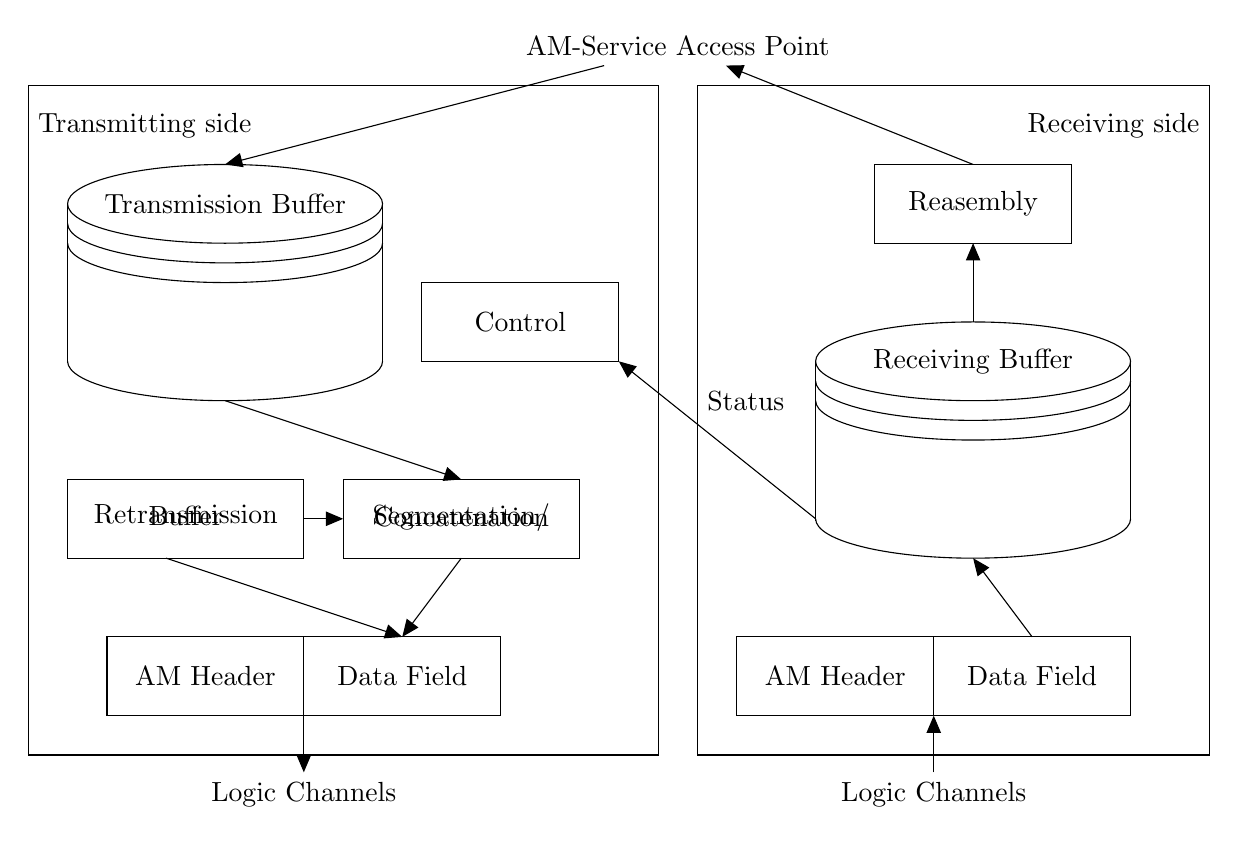
\begin{tikzpicture}[scale=.5]

\draw  (-1,9) rectangle (-17,-8);
\draw  (0,9) rectangle (13,-8);

\node (v1) at (-12,6) {Transmission Buffer};
\draw  (v1) ellipse (4 and 1);
\draw (-16,5.5) arc (180:360:4 and 1);
\draw (-16,5) arc (180:360:4 and 1);
\draw (-16,2) arc (180:360:4 and 1);
\node (v2) at (-16,6) {};
\node (v4) at (-8,6) {};
\node (v3) at (-16,1.7) {};
\node (v5) at (-8,1.7) {};
\draw  (v2) ++(0,0) edge (v3);
\draw  (v4)  ++(0,0) edge (v5);

\draw  (-9,-1) rectangle (-3,-3);
\node at (-6,-2) {\begin{tabular}{c} Segmentation/ \\[-0.9em] Concatenation\end{tabular}};
\draw  (-15,-5) rectangle (-10,-7) node (v6) {};
\draw  (v6) rectangle (-5,-5);
\node at (-12.5,-6) {AM Header};
\node at (-7.5,-6) {Data Field};



\node (v10) at (7,2) {Receiving Buffer};
\draw  (v10) ellipse (4 and 1);
\draw (3,1.5) arc (180:360:4 and 1);
\draw (3,1) arc (180:360:4 and 1);
\draw (3,-2) node (v23) {} arc (180:360:4 and 1);
\node (v20) at (3,2) {};
\node (v40) at (11,2) {};
\node (v30) at (3,-2.3) {};
\node (v50) at (11,-2.3) {};
\draw  (v20) ++(0,0) edge (v30);
\draw  (v40)  ++(0,0) edge (v50);


\draw  (4.5,7) rectangle (9.5,5);
\draw  (1,-5) rectangle (6,-7) node (v7) {};
\draw  (v7) rectangle (11,-5);
\node at (7,6) {Reasembly};
\node at (7,-1.5) {};
\node at (3.5,-6) {AM Header};
\node at (8.5,-6) {Data Field};

\node (v15) at (-10,-9) {Logic Channels};
\node (v16) at (6,-9) {Logic Channels};
\node (v14) at (-7.5,-5) {};
\node (v13) at (-6,-3) {};
\node (v11) at (-12,1) {};
\node (v9) at (-12,7) {};
\node (v8) at (-0.5,10) {AM-Service Access Point};
\node (v22) at (7,7) {};
\node (v21) at (7,5) {};
\node (v19) at (7,3) {};
\node (v18) at (7,-3) {};
\node (v17) at (8.5,-5) {};
\node (v12) at (-6,-1) {};

\draw [arrows={ - triangle 45}] (v8) -- (-12,7);
\draw [arrows={ - triangle 45}] (-12,1) -- (-6,-1);
\draw [arrows={ - triangle 45}] (-6,-3) -- (-7.5,-5);
\draw [arrows={ - triangle 45}] (-10,-7) -- (v15);
\draw [arrows={ - triangle 45}] (v16) -- (6,-7);
\draw [arrows={ - triangle 45}] (8.5,-5) -- (7,-3);
\draw [arrows={ - triangle 45}] (7,3) -- (7,5);
\draw [arrows={ - triangle 45}] (7,7) -- (v8);
\node [anchor=west] at (-17,8) {Transmitting side};
\node [anchor=east] at (13,8) {Receiving side};
\draw  (-10,-1) rectangle (-16,-3);
\node at (-13,-2) {\begin{tabular}{c} Retransmission \\[-0.9em] Buffer\end{tabular}};
\draw  (-7,4) rectangle (-2,2) node (v24) {};
\node at (-4.5,3) {Control};
\draw [arrows={ - triangle 45}] (3,-2) -- (-2,2);
\node [anchor=west] at (0,1) {Status};
\node (v25) at (-10.2,-2) {};
\node (v26) at (-8.8,-2) {};
\node (v27) at (-13.5,-3) {};
\draw [arrows={ - triangle 45}] (-10,-2) -- (-9,-2);
\draw [arrows={ - triangle 45}] (-13.5,-3) -- (-7.5,-5);
\end{tikzpicture}}
\caption{\gls{RLC} \gls{AM} operation \citep[ch. 6.4]{book_LTE_for_UMTS}}
\label{fig:RLC_AM/UM_operation}
\end{figure}
\end{minipage}
\captionsetup{belowskip=-1.5em}

In \gls{LTE} several logic channels are defined in the \gls{RLC} layer three for uplink and five for downlink \citep[ch. 6.3]{book_LTE_for_UMTS}. 

Common logical channels:
\begin{itemize}
\item The \gls{CCCH} is used to transport control information before a \gls{RRC} connection exist.  
\item The \gls{DCCH} is used to transport control information after a \gls{RRC} connection is established. 
\item The \gls{DTCH} is used to carry user data.
\end{itemize}
Downlink specific logical channels:
\begin{itemize}
\item The \gls{BCCH} is used to carry the system information and other system access related information.
\item The \gls{PCCH} is used to carry paging information to reach \gls{UE}s that are not in connected mode.
%\item The \gls{MCCH}
%\item \gls{MTCH}
\end{itemize}
%\todo{missing something about the logical channels CCCH DCCH DTCH PCCH BCCH MCCH MTCH}

\subsection{MAC}

The \gls{MAC} layer takes care of several things first of it maps the logical channels to the transport channels. Five transport channels are defined: the \gls{RACH}, the \gls{UL-SCH}, the \gls{DL-SCH} the \gls{BCH} and the \gls{PCH}. All logical channels are mapped to these depending on the direction of the information as can be seen in \autoref{fig:MAC_PDU_DL} and \autoref{fig:MAC_PDU_UL}. The \gls{RACH} handles the random access procedure this is solely a \gls{MAC} layer functionality there are therefore no logic channel mapped to it. The \gls{MAC} layer further handles multiplexing/demultiplexing of \gls{RLC} \gls{PDU}s into \gls{TB} for the physical layer including padding if a \gls{PDU} is not completely filled with data. It also handles traffic volume measurement and reporting and provides this information for the \gls{RRC} layer. Another function the \gls{MAC} layer handles is the error correction through \gls{HARQ} along with scheduling of the physical layer. The final thing the \gls{MAC} layer handles is the transport format selection, this includes \gls{AL}, \gls{MCS} and power ramping.  

\captionsetup{belowskip=0em}
\begin{minipage}{0.48\textwidth}
	\tikzsetnextfilename{MAC_DL-mapping}
	\begin{figure}[H]
	\centering
	\resizebox{\textwidth}{!}{
	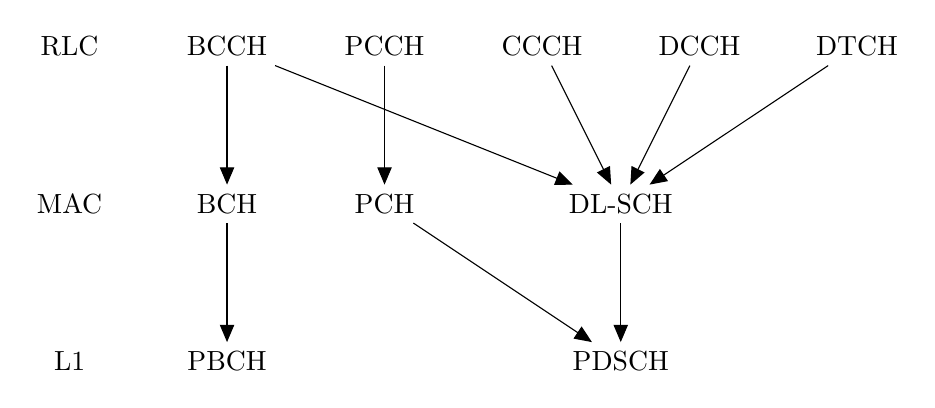
\begin{tikzpicture}[scale=.5]

\node at (-10,5) {RLC};
\node at (-10,1) {MAC};
\node at (-10,-3) {L1};

\node (v1) at (-6,5) {BCCH};
\node (v2) at (-6,1) {BCH};
\node (v3) at (-6,-3) {PBCH};

\node (v5) at (-2,5) {PCCH};
\node (v6) at (-2,1) {PCH};

\node (v8) at (2,5) {CCCH};

\node (v9) at (6,5) {DCCH};

\node (v10) at (10,5) {DTCH};
\node (v4) at (4,1) {DL-SCH};
\node (v7) at (4,-3) {PDSCH};

%\node (v11) at (14,5) {MCCH};
%
%\node (v12) at (18,5) {MTCH};
%\node (v13) at (18,1) {MCH};
%\node (v14) at (18,-3) {PMCH};

\draw [arrows={-triangle 45}] (v1) edge (v2);
\draw [arrows={-triangle 45}] (v2) edge (v3);
\draw [arrows={-triangle 45}] (v1) edge (v4);
\draw [arrows={-triangle 45}] (v5) edge (v6);
\draw [arrows={-triangle 45}] (v6) edge (v7);
\draw [arrows={-triangle 45}] (v8) edge (v4);
\draw [arrows={-triangle 45}] (v9) edge (v4);
\draw [arrows={-triangle 45}] (v10) edge (v4);
\draw [arrows={-triangle 45}] (v4) edge (v7);
%\draw [arrows={-triangle 45}] (v11) edge (v4);
%\draw [arrows={-triangle 45}] (v12) edge (v4);
%\draw [arrows={-triangle 45}] (v12) edge (v13);
%\draw [arrows={-triangle 45}] (v13) edge (v14);
\end{tikzpicture}}
	\caption{\gls{MAC} layer \gls{DL} mapping structure}
	\label{fig:MAC_PDU_DL}
	\end{figure}
\end{minipage}
\begin{minipage}{0.48\textwidth}
	\tikzsetnextfilename{MAC_UL-mapping}
	\begin{figure}[H]
	\centering
	\resizebox{\textwidth}{!}{
	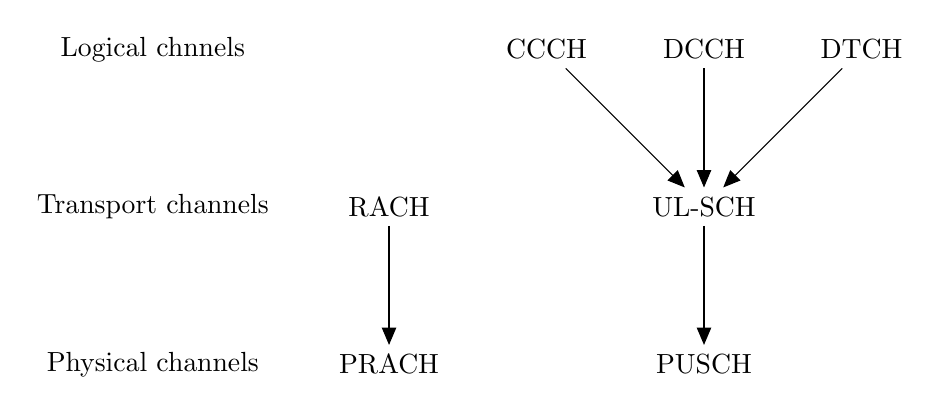
\begin{tikzpicture}[scale=.5]

\node at (-10,5) {Logical chnnels};
\node at (-10,1) {Transport channels};
\node at (-10,-3) {Physical channels};

\node (v1) at (-4,1) {RACH};
\node (v2) at (-4,-3) {PRACH};

\node (v3) at (0,5) {CCCH};

\node (v4) at (4,5) {DCCH};

\node (v5) at (8,5) {DTCH};
\node (v6) at (4,1) {UL-SCH};
\node (v7) at (4,-3) {PUSCH};


\draw [arrows={-triangle 45}] (v1) edge (v2);
\draw [arrows={-triangle 45}] (v3) edge (v6);
 \draw [arrows={-triangle 45}] (v4) edge (v6);
 \draw [arrows={-triangle 45}] (v5) edge (v6);
 \draw [arrows={-triangle 45}] (v6) edge (v7);
\end{tikzpicture}}
	\caption{\gls{MAC} layer \gls{UL} mapping structure}
	\label{fig:MAC_PDU_UL}
	\end{figure}
\end{minipage}
\captionsetup{belowskip=-1.5em}

A \gls{MAC} \gls{PDU} consist of the \gls{MAC} header along with the \gls{MAC} control elements and the \gls{MAC} \gls{SDU}s and potentially some padding as can be seen in \autoref{fig:MAC_PDU}

\tikzsetnextfilename{MAC_PDU}
\begin{figure}[H]
\centering
\resizebox{\textwidth}{!}{
\usetikzlibrary{decorations.pathreplacing}
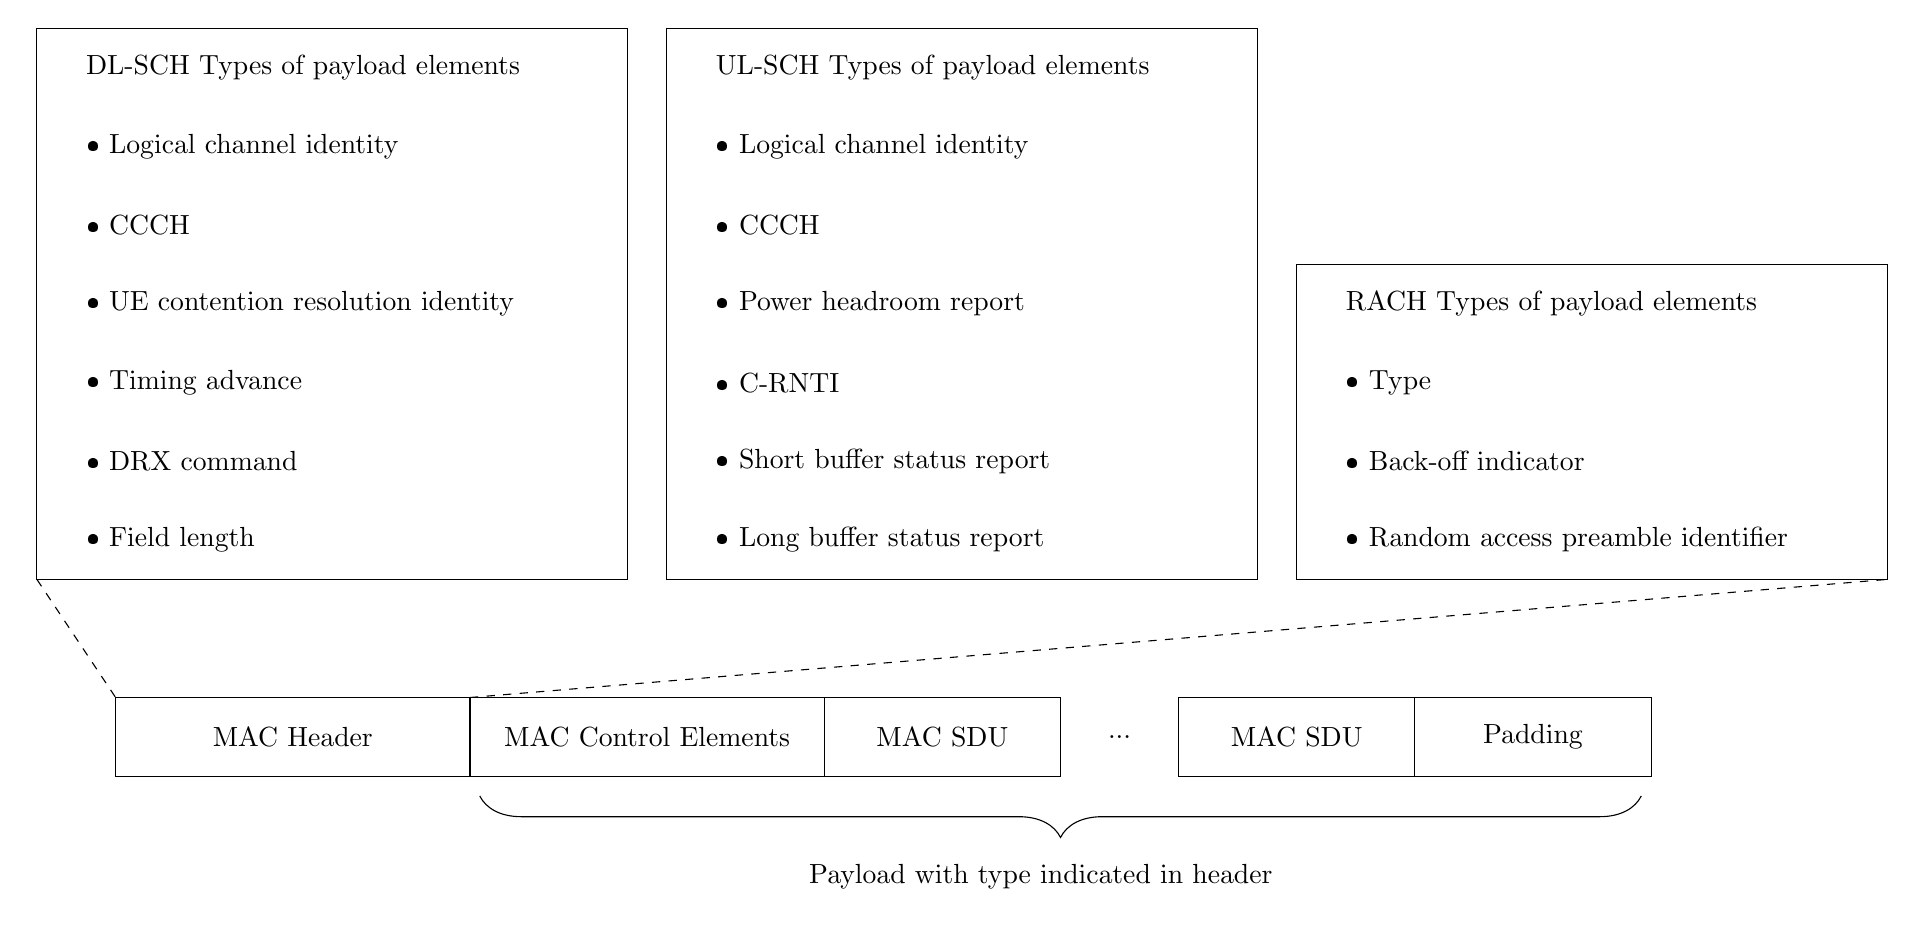
\begin{tikzpicture}[scale=.5]

\draw  (-10,8) rectangle (5,-6);
\node [anchor=west] at (-9,7) {DL-SCH Types of payload elements};
\node [anchor=west] at (-9,5) {• Logical channel identity};
\node [anchor=west] at (-9,3) {• CCCH};
\node [anchor=west] at (-9,1) {• UE contention resolution identity};
\node [anchor=west] at (-9,-1) {• Timing advance};
\node [anchor=west] at (-9,-3) {• DRX command};
\node [anchor=west] at (-9,-5) {• Field length};

\draw  (6,8) rectangle (21,-6) {};
\node [anchor=west] at (7,7) {UL-SCH Types of payload elements};
\node [anchor=west] at (7,5) {• Logical channel identity};
\node [anchor=west] at (7,3) {• CCCH};
\node [anchor=west] at (7,1) {• Power headroom report};
\node [anchor=west] at (7,-1) {• C-RNTI};
\node [anchor=west] at (7,-3) {• Short buffer status report};
\node [anchor=west] at (7,-5) {• Long buffer status report};

\draw  (22,2) rectangle (37,-6) node (v4) {};
\node [anchor=west] at (23,1) {RACH Types of payload elements};
\node [anchor=west] at (23,-1) {• Type};
\node [anchor=west] at (23,-3) {• Back-off indicator};
\node [anchor=west] at (23,-5) {• Random access preamble identifier};

\draw  (-8,-9) node (v2) {} rectangle (1,-11);
\node at (-3.5,-10) {MAC Header};
\draw  (1,-9) node (v3) {} rectangle (10,-11);
\node at (5.5,-10) {MAC Control Elements};
\draw  (10,-9) rectangle (16,-11);
\node at (13,-10) {MAC SDU};
\node at (17.5,-10) {...};
\draw  (19,-9) rectangle (25,-11);
\node at (22,-10) {MAC SDU};
\draw  (25,-9) rectangle (31,-11);
\node at (28,-10) {Padding};

\node (v1) at (-10,-6) {};
\draw [dashed] (-10,-6) -- (-8,-9);
\draw [dashed] (1,-9) -- (37,-6);
\node (v5) at (1,-11.5) {};
\node (v6) at (31,-11.5) {};
\draw [decorate,decoration={brace,amplitude=15pt}] (v6) -- (v5);
\node [anchor=north] at (15.5,-13) {Payload with type indicated in header};
\end{tikzpicture}}
\caption{MAC PDU structure}
\label{fig:MAC_PDU}
\end{figure}

The header is different depending upon which transport channel is used as can be seen in \autoref{fig:MAC_PDU}. It include key parameter for control of both the physical layer as well as the logical channel identity. It is also the \gls{MAC} layer that handles contention resolution with \gls{HARQ}, for this purpose the header includes \gls{CCCH} and \gls{C-RNTI} for the device. When a device tries to connect to the network the \gls{MAC} layer also calculates timing advance. 


\subsection{PHY}\label{sec:NB-IoT/Physical Layer}

To accommodate the new requirements set by the \gls{IoT} development as described in the beginning of \autoref{ch:NB-IoT}, the physical layer design also needs to be revised. The idea is to allow for three different deployments methods: in-band, guard-band and standalone \citep{primer}. This is to take advantage of the existing \gls{LTE} and \gls{GSM} networks. The idea behind the three deployments can be seen in \autoref{fig:NB deployment}, the in-band mode takes up one of the \gls{PRB} from the \gls{LTE} cell, where the guard-band mode places it just outside the LTE carriers. This is possible because none of the \gls{LTE} cells utilize the entire allocated spectrum to reduce the spectral disturbance. The proposed design also allows for the standalone case to utilize a \gls{GSM} band taking advantage of the lower frequency compared to legacy \gls{LTE} to increase the coverage area. To work inside and alongside these system provides some restrictions that needs to be respected. Therefore is the physical structure of the system the same for all deployment methods, however the use and spectrum allocation differs slightly. The most commonly discussed deployment scenario is the in-band operation as this set the most restriction for the \gls{NB-IoT} system. \citep{REL-13,primer}. 

\begin{figure}[H]
\centering
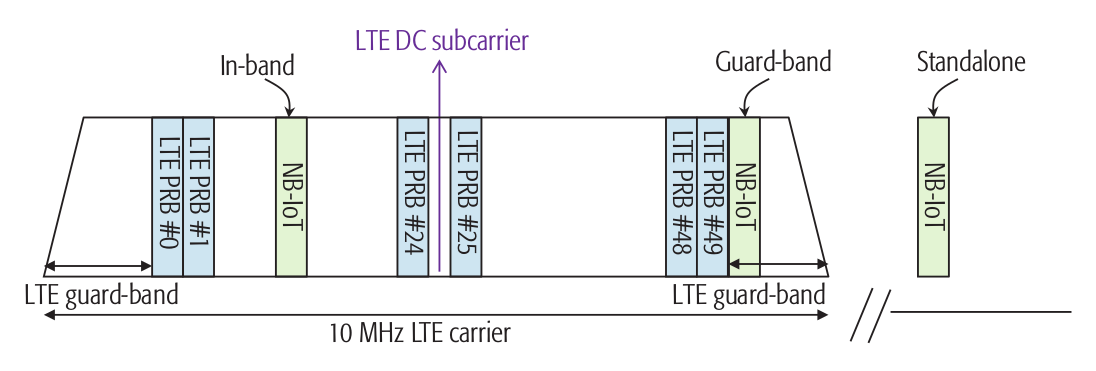
\includegraphics[width=\textwidth]{figures/deployment.png}
\caption{Deployment of the NB-IoT as in-band, guard-band or standalone \citep{primer}.}
\label{fig:NB deployment}
\end{figure}

To allow in-band operation the physical layer of \gls{NB-IoT} needs to follow the overall structure of \gls{LTE}, to describe this it is split into the \gls{DL} and \gls{UL} part. First the \gls{DL} part will be investigated as this accounts for most of the critical factors of the communication i.e. synchronization and system information. 

\subsubsection{Downlink}
As the primary users of legacy \gls{LTE} does not know of the \gls{NB-IoT} system the primary concern is the interference it causes. Some structural guidelines is therefore needed when designing the \gls{NB-IoT} system, first it needs to blend in with the \gls{OFDM} symbols of the \gls{LTE} system meaning that timing alignment and subcarrier spacing is already determined \citep[ch. 7.2]{NB-IoT_Book}. 

Channel Raster\\
As \gls{NB-IoT} functions as an individual system it needs it own overhead. To ensure the functionality of both systems the \gls{PRB}s used for \gls{NB-IoT} is therefore placed outside the six center \gls{PRB}'s, as these are used for LTE synchronization. This implies that only the LTE cells with a bandwidth larger than 1.4 MHz can host NB-IoT \citep{whitepaper}. Furthermore to keep the receiver complexity and the battery consumption at a minimum the \gls{UE} searches for the \gls{NB-IoT} cell on a raster of 100 kHz \citep[ch. 7.2]{NB-IoT_Book}. The center of the bandwidth host a DC-subcarrier, and the \gls{PRB}'s is placed around this. This means that the center of a PRB will be offset from the raster for instance PRB \#25 in \autoref{fig:NB deployment} has a center of 97.5 kHz which is 2.5 kHz off from the raster. Because of this an additional requirement is made that only those \gls{PRB}'s where the offset is less than 7.5 kHz can be used to host a NB-IoT cell \citep{primer}. The PRB's that fulfil this criteria can be seen in \autoref{tab:available-PRBs}. 

\begin{table}[H]
\centering
\begin{tabular}{|c|p{1.8cm}|p{1.8cm}|p{1.8cm}|p{1.8cm}|p{1.8cm}|}\hline
\textbf{LTE cell bandwidth}	& 3 MHz				& 5 MHz	& 10 MHz	& 15 MHz	& 20 MHz \\\hline
Available PRB indexes		& 2, 12	& 2, 7, 17, 22	& 4, 9, 14, 19, 30, 35, 40, 45 & 2, 7, 12, 17, 22, 27, 32, 42, 47, 52, 57, 62, 67, 72 & 4, 9, 14, 19, 24, 29, 34, 39, 44, 55, 60, 65, 70, 75, 80, 85, 90, 95 \\\hline
\end{tabular}
\caption{available-PRBs \citep{whitepaper}}
\label{tab:available-PRBs}
\end{table}


Frame Structure\\
To fit into a \gls{LTE} \gls{PRB} the frame structure needs to be very similar to legacy \gls{LTE}, the structure is divided into: hyperframe, frame, subframe and slots. Where two slots make a subframe, ten subframes make a frame and 1024 frames make a hyperframe. A complete cycle takes 1024 hyperframes which corresponds to 2 hours 54 minutes and 46 seconds.  \autoref{fig:downlink-structure} \citep[ch. 7.2]{NB-IoT_Book}. 


\begin{figure}[H]
\centering
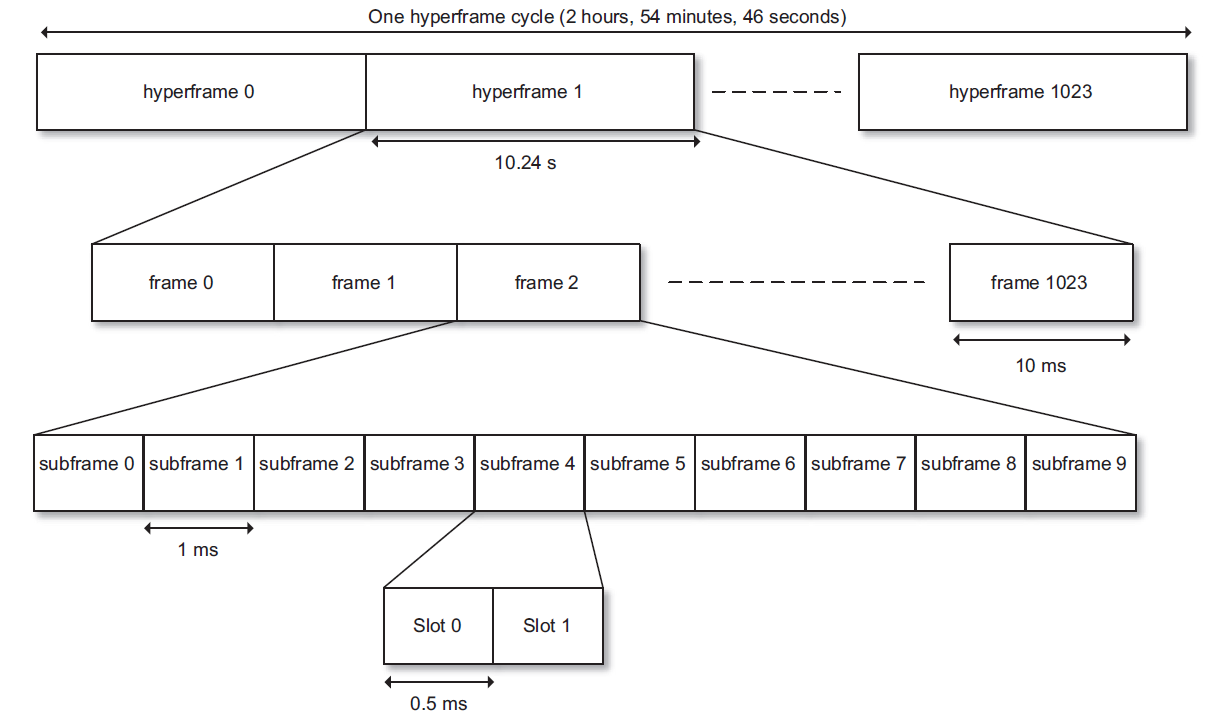
\includegraphics[width=\textwidth]{figures/downlink_structure_15kHz.png}
\caption{\gls{NB-IoT} downlink structure \citep[Fig. 7.7]{NB-IoT_Book}}
\label{fig:downlink-structure}
\end{figure}


As the \gls{NB-IoT} system is placed outside the \gls{PRB}s used for LTE synchronization most of the subframes are available to use, the only exception is if a \gls{MBSFN} is present, this can occupy either of subframes (1,2,3,6,7,8) \citep{LTE-MBSFN}. Therefore the \gls{NPSS} and \gls{NSSS} is placed in subframe 5 and 9 respectively as seen in \autoref{fig:frame-structure}. By having the \gls{NSSS} being present only in even frame numbers, the \gls{LSB} of the frame numbers can be deduced directly, this increases the efficiency of the system by freeing subframe 9 in odd frames and omitting that bit from the \gls{NB-IoT} overhead. The \gls{NPBCH} is located in the subframe 0 and contains the \gls{MIB-NB} which was explained in \autoref{sec:RRC} \citep{REL-13}.  

\tikzsetnextfilename{frameStructure}
\begin{figure}[H]
\centering
\definecolor{NPSS}{HTML}{00D0FF}
\definecolor{NSSS}{HTML}{F97BFF}
\definecolor{NPBCH}{HTML}{92D050}
\usetikzlibrary{patterns,decorations.pathreplacing}

\resizebox{\textwidth}{!}{
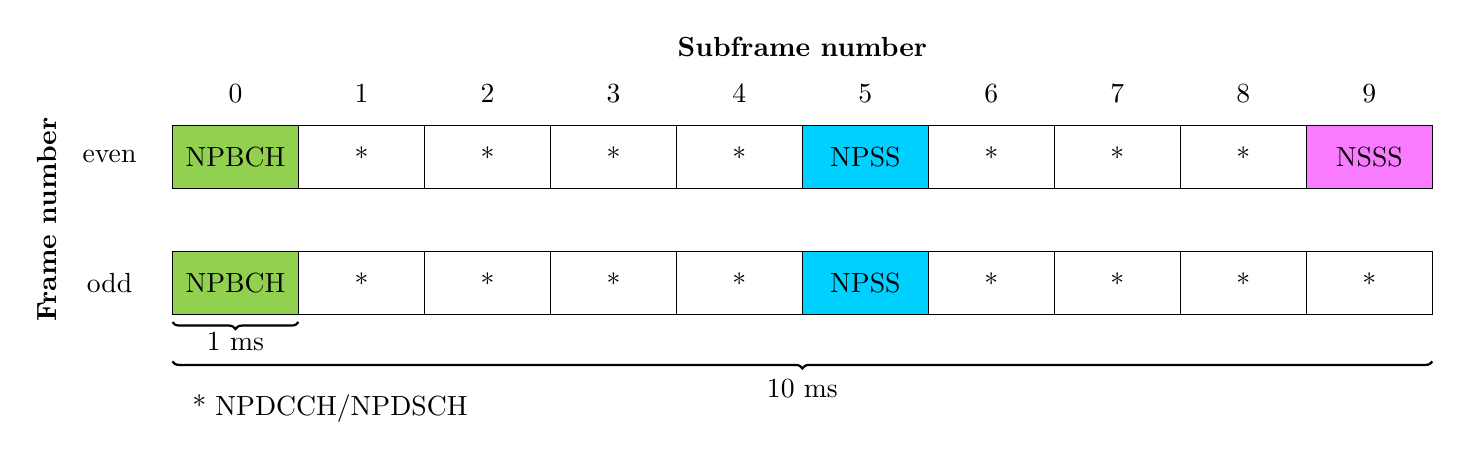
\begin{tikzpicture}[scale = 0.4]

\draw [thick,decoration={brace,mirror,raise=0.1cm},decorate] (-20,-4) -- (-16,-4) node [pos=0.5,anchor=north,yshift=-0.1cm] {1 ms}; 
\draw [thick,decoration={brace,mirror,raise=0.2cm},decorate] (-20,-5) -- (20,-5) node [pos=0.5,anchor=north,yshift=-0.3cm] {10 ms};



\draw[fill = NPBCH]  (-20,2) rectangle (-16,0);
\draw  (-16,2) rectangle (-12,0);
\draw  (-12,2) rectangle (-8,0);
\draw  (-8,2) rectangle (-4,0);
\draw  (-4,2) rectangle (0,0);
\draw[fill = NPSS]  (0,2) rectangle (4,0);
\draw  (4,2) rectangle (8,0);
\draw  (8,2) rectangle (12,0);
\draw  (12,2) rectangle (16,0);
\draw[fill = NSSS]  (16,2) rectangle (20,0);

\draw[fill = NPBCH]  (-20,-2) rectangle (-16,-4);
\draw  (-16,-2) rectangle (-12,-4);
\draw  (-12,-2) rectangle (-8,-4);
\draw  (-8,-2) rectangle (-4,-4);
\draw  (-4,-2) rectangle (0,-4);
\draw[fill = NPSS]  (0,-2) rectangle (4,-4);
\draw  (4,-2) rectangle (8,-4);
\draw  (8,-2) rectangle (12,-4);
\draw  (12,-2) rectangle (16,-4);
\draw  (16,-2) rectangle (20,-4);

\node at (-18,3) {0};
\node at (-14,3) {1};
\node at (-10,3) {2};
\node at (-6,3) {3};
\node at (-2,3) {4};
\node at (2,3) {5};
\node at (6,3) {6};
\node at (10,3) {7};
\node at (14,3) {8};
\node at (18,3) {9};
\node at (-22,1) {even};
\node at (-22,-3) {odd};
\node [rotate = 90] at (-24,-1) {\textbf{Frame number}}; 

\node at (-18,1) {\acrshort{NPBCH}};
\node at (-18,-3) {\acrshort{NPBCH}};
\node at (2,1) {\acrshort{NPSS}};
\node at (2,-3) {\acrshort{NPSS}};
\node at (18,1) {\acrshort{NSSS}};
\node at (-14,1) {*};
\node at (-10,1) {*};
\node at (-6,1) {*};
\node at (-2,1) {*};
\node at (6,1) {*};
\node at (10,1) {*};
\node at (14,1) {*};
\node at (-14,-3) {*};
\node at (-10,-3) {*};
\node at (-6,-3) {*};
\node at (-2,-3) {*};
\node at (6,-3) {*};
\node at (10,-3) {*};
\node at (14,-3) {*};
\node at (18,-3) {*};
\node at (0,4.5) {\textbf{Subframe number}}; 

\node at (-15,-7) {* \acrshort{NPDCCH}/\acrshort{NPDSCH}};
\end{tikzpicture}
}

\caption{\gls{NB-IoT} frame structure \citep{REL-13}}
\label{fig:frame-structure}
\end{figure}


By zooming in on a subframe, it is possible to see how the different \gls{OFDM} symbols is utilized. During a subframe 14 \gls{OFDM} symbols are transmitted each having 12 subcarriers. As can be seen from \autoref{fig:subframe-structure} almost half of the \gls{RE} in a subframe might be reserved for different signals and \gls{LTE} control information \citep{REL-13}. An \gls{LTE} cell can allocate up to three symbols for \gls{PDCCH}, an might use up to four carriers needing four \gls{RS}s \citep{whitepaper}. The \gls{NB-IoT} structure allows for up to two carriers and needs therefore two \gls{RS} namely \gls{NRS}1 and \gls{NRS}2 \citep{REL-13}. The placement of all these signals can be seen in \autoref{fig:subframe-structure}.  

\tikzsetnextfilename{subframe}
\begin{figure}[H]
\centering
\definecolor{LTERS}{HTML}{496d22}
\definecolor{LTECCH}{HTML}{92D050}
\definecolor{NPSS}{HTML}{00D0FF}
\definecolor{NSSS}{HTML}{F97BFF}


\resizebox{\textwidth}{!}{
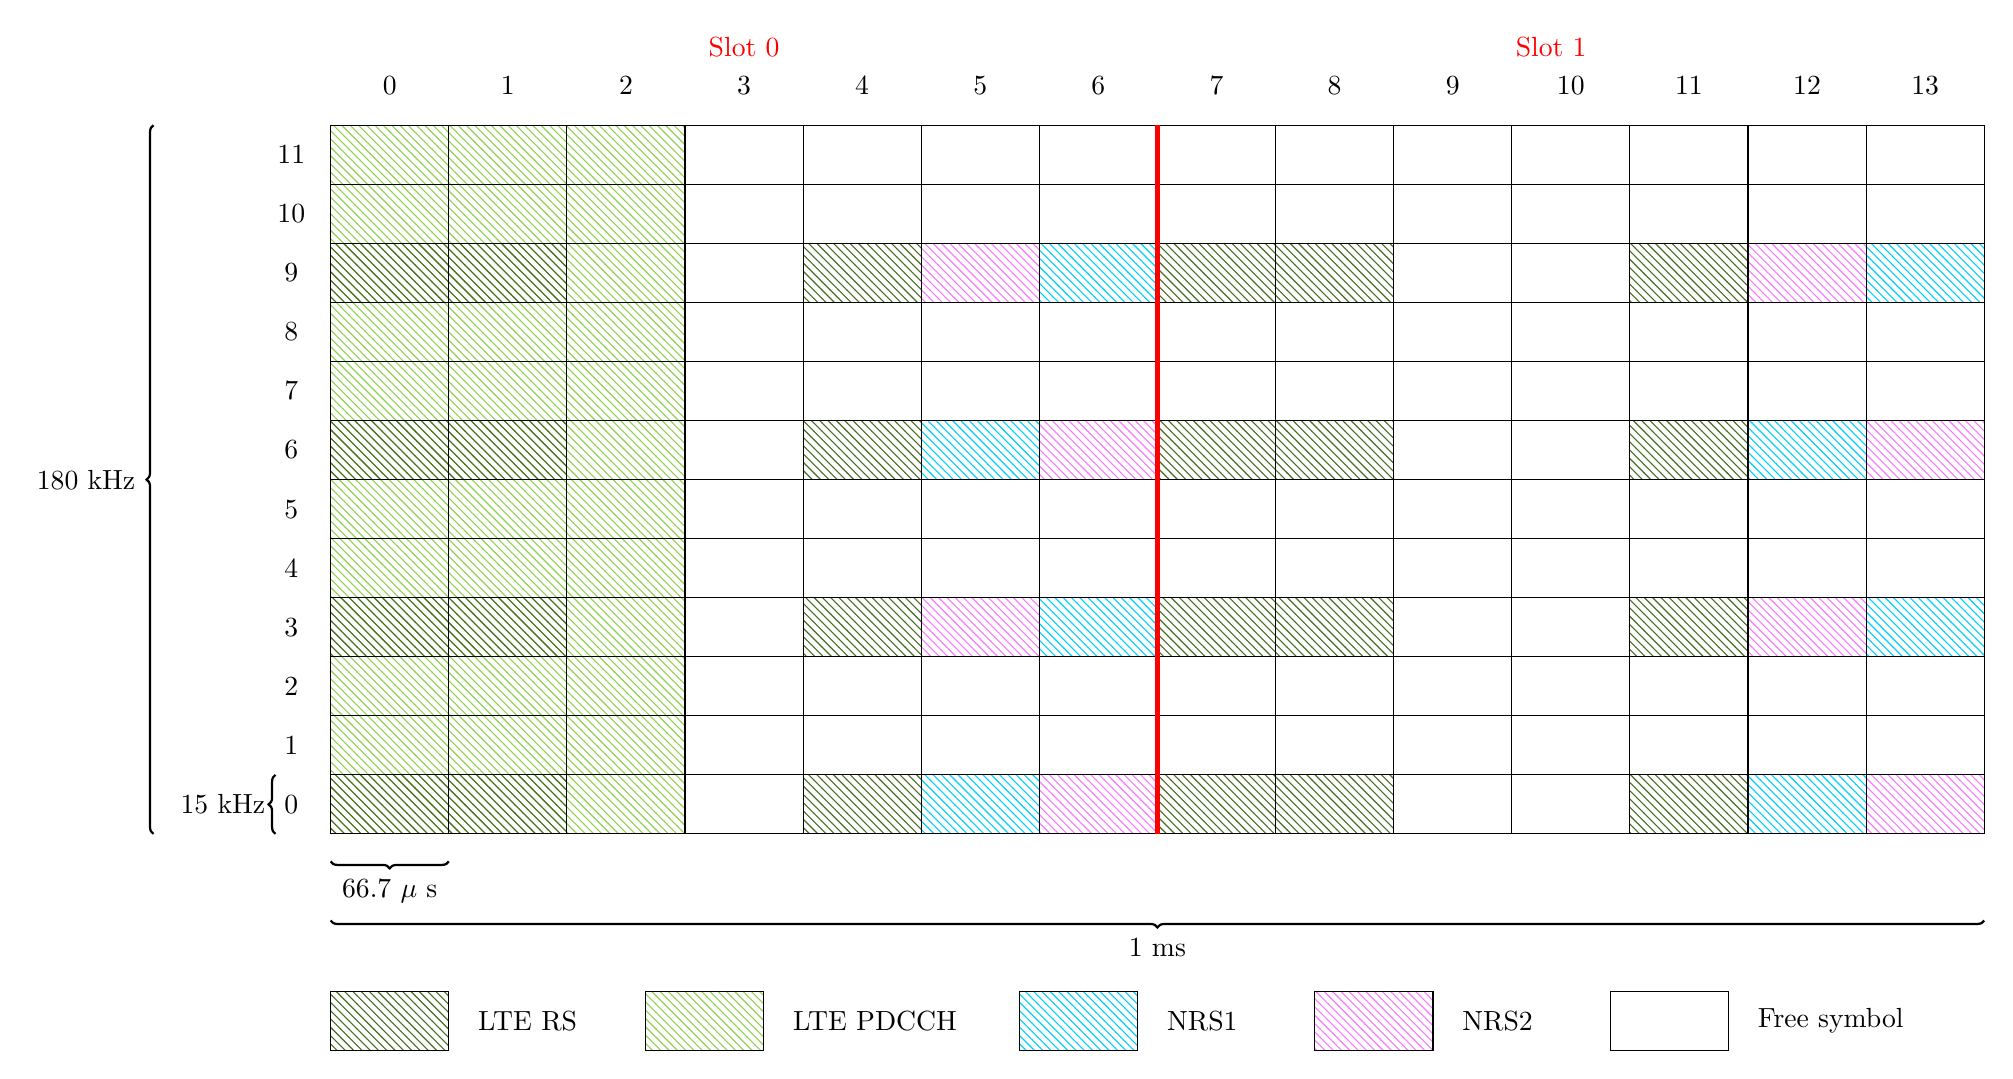
\begin{tikzpicture}[scale=0.5]

\draw[pattern=north west lines, pattern color=LTECCH]  (-21,9) rectangle (-12,-9);
\draw [thick,decoration={brace,mirror},decorate] (-25.5,9) -- (-25.5,-9) node [pos=0.5,anchor=east, xshift=-0.1cm] {180 kHz};
\draw [thick,decoration={brace,mirror,raise=0.1cm},decorate] (-22.2,-7.5) -- (-22.2,-9) node [pos=0.5,anchor=east,xshift=-0.1cm] {15 kHz};
\draw [thick,decoration={brace,mirror,raise=0.1cm},decorate] (-21,-9.5) -- (-18,-9.5) node [pos=0.5,anchor=north,yshift=-0.2cm] {66.7 $\mu$ s};
\draw [thick,decoration={brace,mirror,raise=0.1cm},decorate] (-21,-11) -- (21,-11) node [pos=0.5,anchor=north,yshift=-0.2cm] {1 ms};


\node[text =red] at (-10.5,11) {Slot 0};
\node[text =red] at (10,11) {Slot 1};

%række 11
\draw  (-21,9) rectangle (-18,7.5);
\draw  (-18,9) rectangle (-15,7.5);
\draw  (-15,9) rectangle (-12,7.5);
\draw  (-12,9) rectangle (-9,7.5);
\draw  (-9,9) rectangle (-6,7.5);
\draw  (-6,9) rectangle (-3,7.5);
\draw  (-3,9) rectangle (0,7.5);
\draw  (-0,9) node (v1) {} rectangle (3,7.5);
\draw  (3,9) rectangle (6,7.5);
\draw  (6,9) rectangle (9,7.5);
\draw  (9,9) rectangle (12,7.5);
\draw  (12,9) rectangle (15,7.5);
\draw  (15,9) rectangle (18,7.5);
\draw  (18,9) rectangle (21,7.5);

%række 10
\draw  (-21,7.5) rectangle (-18,6);
\draw  (-18,7.5) rectangle (-15,6);
\draw  (-15,7.5) rectangle (-12,6);
\draw  (-12,7.5) rectangle (-9,6);
\draw  (-9,7.5) rectangle (-6,6);
\draw  (-6,7.5) rectangle (-3,6);
\draw  (-3,7.5) rectangle (0,6);
\draw  (-0,7.5) rectangle (3,6);
\draw  (3,7.5) rectangle (6,6);
\draw  (6,7.5) rectangle (9,6);
\draw  (9,7.5) rectangle (12,6);
\draw  (12,7.5) rectangle (15,6);
\draw  (15,7.5) rectangle (18,6);
\draw  (18,7.5) rectangle (21,6);

%række 9
\draw[pattern=north west lines, pattern color=LTERS] (-21,6) rectangle (-18,4.5);
\draw[pattern=north west lines, pattern color=LTERS] (-18,6) rectangle (-15,4.5);
\draw  (-15,6) rectangle (-12,4.5);
\draw  (-12,6) rectangle (-9,4.5);
\draw[pattern=north west lines, pattern color=LTERS]  (-9,6) rectangle (-6,4.5);
\draw[pattern=north west lines, pattern color=NSSS]  (-6,6) rectangle (-3,4.5);
\draw[pattern=north west lines, pattern color=NPSS]  (-3,6) rectangle (0,4.5);
\draw[pattern=north west lines, pattern color=LTERS]  (-0,6) rectangle (3,4.5);
\draw[pattern=north west lines, pattern color=LTERS]  (3,6) rectangle (6,4.5);
\draw  (6,6) rectangle (9,4.5);
\draw  (9,6) rectangle (12,4.5);
\draw[pattern=north west lines, pattern color=LTERS]  (12,6) rectangle (15,4.5);
\draw[pattern=north west lines, pattern color=NSSS] (15,6) rectangle (18,4.5);
\draw[pattern=north west lines, pattern color=NPSS]  (18,6) rectangle (21,4.5);

%række 8
\draw  (-21,4.5) rectangle (-18,3);
\draw  (-18,4.5) rectangle (-15,3);
\draw  (-15,4.5) rectangle (-12,3);
\draw  (-12,4.5) rectangle (-9,3);
\draw  (-9,4.5) rectangle (-6,3);
\draw  (-6,4.5) rectangle (-3,3);
\draw  (-3,4.5) rectangle (0,3);
\draw  (-0,4.5) rectangle (3,3);
\draw  (3,4.5) rectangle (6,3);
\draw  (6,4.5) rectangle (9,3);
\draw  (9,4.5) rectangle (12,3);
\draw  (12,4.5) rectangle (15,3);
\draw  (15,4.5) rectangle (18,3);
\draw  (18,4.5) rectangle (21,3);

%række 7
\draw  (-21,3) rectangle (-18,1.5);
\draw  (-18,3) rectangle (-15,1.5);
\draw  (-15,3) rectangle (-12,1.5);
\draw  (-12,3) rectangle (-9,1.5);
\draw  (-9,3) rectangle (-6,1.5);
\draw  (-6,3) rectangle (-3,1.5);
\draw  (-3,3) rectangle (0,1.5);
\draw  (-0,3) rectangle (3,1.5);
\draw  (3,3) rectangle (6,1.5);
\draw  (6,3) rectangle (9,1.5);
\draw  (9,3) rectangle (12,1.5);
\draw  (12,3) rectangle (15,1.5);
\draw  (15,3) rectangle (18,1.5);
\draw  (18,3) rectangle (21,1.5);

%række 6
\draw[pattern=north west lines, pattern color=LTERS] (-21,1.5) rectangle (-18,0);
\draw[pattern=north west lines, pattern color=LTERS] (-18,1.5) rectangle (-15,0);
\draw  (-15,1.5) rectangle (-12,0);
\draw  (-12,1.5) rectangle (-9,0);
\draw[pattern=north west lines, pattern color=LTERS]  (-9,1.5) rectangle (-6,0);
\draw[pattern=north west lines, pattern color=NPSS]  (-6,1.5) rectangle (-3,0);
\draw[pattern=north west lines, pattern color=NSSS]  (-3,1.5) rectangle (0,0);
\draw[pattern=north west lines, pattern color=LTERS]  (-0,1.5) rectangle (3,0);
\draw[pattern=north west lines, pattern color=LTERS]  (3,1.5) rectangle (6,0);
\draw  (6,1.5) rectangle (9,0);
\draw  (9,1.5) rectangle (12,0);
\draw[pattern=north west lines, pattern color=LTERS]  (12,1.5) rectangle (15,0);
\draw[pattern=north west lines, pattern color=NPSS]  (15,1.5) rectangle (18,0);
\draw[pattern=north west lines, pattern color=NSSS] (18,1.5) rectangle (21,0);

%række 5
\draw  (-21,-0) rectangle (-18,-1.5);
\draw  (-18,-0) rectangle (-15,-1.5);
\draw  (-15,-0) rectangle (-12,-1.5);
\draw  (-12,-0) rectangle (-9,-1.5);
\draw  (-9,-0) rectangle (-6,-1.5);
\draw  (-6,-0) rectangle (-3,-1.5);
\draw  (-3,-0) rectangle (0,-1.5);
\draw  (-0,-0) rectangle (3,-1.5);
\draw  (3,-0) rectangle (6,-1.5);
\draw  (6,-0) rectangle (9,-1.5);
\draw  (9,-0) rectangle (12,-1.5);
\draw  (12,-0) rectangle (15,-1.5);
\draw  (15,-0) rectangle (18,-1.5);
\draw  (18,-0) rectangle (21,-1.5);

%række 4
\draw  (-21,-1.5) rectangle (-18,-3);
\draw  (-18,-1.5) rectangle (-15,-3);
\draw  (-15,-1.5) rectangle (-12,-3);
\draw  (-12,-1.5) rectangle (-9,-3);
\draw  (-9,-1.5) rectangle (-6,-3);
\draw  (-6,-1.5) rectangle (-3,-3);
\draw  (-3,-1.5) rectangle (0,-3);
\draw  (-0,-1.5) rectangle (3,-3);
\draw  (3,-1.5) rectangle (6,-3);
\draw  (6,-1.5) rectangle (9,-3);
\draw  (9,-1.5) rectangle (12,-3);
\draw  (12,-1.5) rectangle (15,-3);
\draw  (15,-1.5) rectangle (18,-3);
\draw  (18,-1.5) rectangle (21,-3);

%række 3
\draw[pattern=north west lines, pattern color=LTERS] (-21,-3) rectangle (-18,-4.5);
\draw[pattern=north west lines, pattern color=LTERS] (-18,-3) rectangle (-15,-4.5);
\draw  (-15,-3) rectangle (-12,-4.5);
\draw  (-12,-3) rectangle (-9,-4.5);
\draw[pattern=north west lines, pattern color=LTERS]  (-9,-3) rectangle (-6,-4.5);
\draw[pattern=north west lines, pattern color=NSSS]  (-6,-3) rectangle (-3,-4.5);
\draw[pattern=north west lines, pattern color=NPSS]  (-3,-3) rectangle (0,-4.5);
\draw[pattern=north west lines, pattern color=LTERS]  (-0,-3) rectangle (3,-4.5);
\draw[pattern=north west lines, pattern color=LTERS]  (3,-3) rectangle (6,-4.5);
\draw  (6,-3) rectangle (9,-4.5);
\draw  (9,-3) rectangle (12,-4.5);
\draw[pattern=north west lines, pattern color=LTERS]  (12,-3) rectangle (15,-4.5);
\draw[pattern=north west lines, pattern color=NSSS]  (15,-3) rectangle (18,-4.5);
\draw[pattern=north west lines, pattern color=NPSS]  (18,-3) rectangle (21,-4.5);

%række 2
\draw  (-21,-4.5) rectangle (-18,-6);
\draw  (-18,-4.5) rectangle (-15,-6);
\draw  (-15,-4.5) rectangle (-12,-6);
\draw  (-12,-4.5) rectangle (-9,-6);
\draw  (-9,-4.5) rectangle (-6,-6);
\draw  (-6,-4.5) rectangle (-3,-6);
\draw  (-3,-4.5) rectangle (0,-6);
\draw  (-0,-4.5) rectangle (3,-6);
\draw  (3,-4.5) rectangle (6,-6);
\draw  (6,-4.5) rectangle (9,-6);
\draw  (9,-4.5) rectangle (12,-6);
\draw  (12,-4.5) rectangle (15,-6);
\draw  (15,-4.5) rectangle (18,-6);
\draw  (18,-4.5) rectangle (21,-6);

%række 1
\draw  (-21,-6) rectangle (-18,-7.5);
\draw  (-18,-6) rectangle (-15,-7.5);
\draw  (-15,-6) rectangle (-12,-7.5);
\draw  (-12,-6) rectangle (-9,-7.5);
\draw  (-9,-6) rectangle (-6,-7.5);
\draw  (-6,-6) rectangle (-3,-7.5);
\draw  (-3,-6) rectangle (0,-7.5);
\draw  (-0,-6) rectangle (3,-7.5);
\draw  (3,-6) rectangle (6,-7.5);
\draw  (6,-6) rectangle (9,-7.5);
\draw  (9,-6) rectangle (12,-7.5);
\draw  (12,-6) rectangle (15,-7.5);
\draw  (15,-6) rectangle (18,-7.5);
\draw  (18,-6) rectangle (21,-7.5);

%række 0
\draw[pattern=north west lines, pattern color=LTERS] (-21,-7.5) rectangle (-18,-9);
\draw[pattern=north west lines, pattern color=LTERS] (-18,-7.5) rectangle (-15,-9);
\draw  (-15,-7.5) rectangle (-12,-9); 
\draw  (-12,-7.5) rectangle (-9,-9);
\draw[pattern=north west lines, pattern color=LTERS]  (-9,-7.5) rectangle (-6,-9);
\draw[pattern=north west lines, pattern color=NPSS]  (-6,-7.5) rectangle (-3,-9);
\draw[pattern=north west lines, pattern color=NSSS]  (-3,-7.5) rectangle (0,-9) node (v2) {};
\draw[pattern=north west lines, pattern color=LTERS]  (-0,-7.5) rectangle (3,-9);
\draw[pattern=north west lines, pattern color=LTERS]  (3,-7.5) rectangle (6,-9);
\draw  (6,-7.5) rectangle (9,-9);
\draw  (9,-7.5) rectangle (12,-9);
\draw[pattern=north west lines, pattern color=LTERS]  (12,-7.5) rectangle (15,-9);
\draw[pattern=north west lines, pattern color=NPSS]  (15,-7.5) rectangle (18,-9);
\draw[pattern=north west lines, pattern color=NSSS]  (18,-7.5) rectangle (21,-9);


\node at (-22,-8.25) {0};
\node at (-22,-6.75) {1};
\node at (-22,-5.25) {2};
\node at (-22,-3.75) {3};
\node at (-22,-2.25) {4};
\node at (-22,-0.75) {5};
\node at (-22,0.75) {6};
\node at (-22,2.25) {7};
\node at (-22,3.75) {8};
\node at (-22,5.25) {9};
\node at (-22,6.75) {10};
\node at (-22,8.25) {11};

\node at (-19.5,10) {0};
\node at (-16.5,10) {1};
\node at (-13.5,10) {2};
\node at (-10.5,10) {3};
\node at (-7.5,10) {4};
\node at (-4.5,10) {5};
\node at (-1.5,10) {6};
\node at (1.5,10) {7};
\node at (4.5,10) {8};
\node at (7.5,10) {9};
\node at (10.5,10) {10};
\node at (13.5,10) {11};
\node at (16.5,10) {12};
\node at (19.5,10) {13};

\draw[draw=red,line width=2pt] (0,9) -- (0,-9);
\draw[pattern=north west lines, pattern color=LTERS]  (-21,-13) rectangle (-18,-14.5);
\draw[pattern=north west lines, pattern color=LTECCH]  (-13,-13) rectangle (-10,-14.5);
\draw[pattern=north west lines, pattern color=NPSS]  (-3.5,-13) rectangle (-0.5,-14.5) ;
\draw[pattern=north west lines, pattern color=NSSS]  (4,-13) rectangle (7,-14.5) ;
\draw (11.5,-13) rectangle (14.5,-14.5);

\node[anchor=west] at (-17.5,-13.75) {\acrshort{LTE} \acrshort{RS}};
\node[anchor=west] at (-9.5,-13.75) {\acrshort{LTE} \acrshort{PDCCH}};
\node[anchor=west] at (-0,-13.75) {\acrshort{NRS}1};
\node[anchor=west] at (7.5,-13.75) {\acrshort{NRS}2};
\node[anchor=west] at (15,-13.75) {Free symbol};

\end{tikzpicture}
}
\caption{subframe structure \citep{whitepaper,REL-13}}
\label{fig:subframe-structure}
\end{figure}

It should be noted that the described allocation is a worst case scenario for the \gls{DL}. If the system is deployed either in guard-band or as stand-alone only the \gls{NRS} is actually used, but before the \gls{UE} is synchronized it does not know what is in use and needs to guard for this worst case scenario. When the \gls{UE} receive the \gls{MIB-NB} and \gls{NB-SIB}1 will it get information in regards to the number of carriers and the size of \gls{LTE} \gls{PDCCH} \citep{whitepaper}. 

Channels\\ 
As shown above three channels exist in the \gls{DL} part of the protocol, these are respectively: \gls{NPBCH}, \gls{NPDCCH} and \gls{NPDSCH}. The structure of the \gls{NPBCH} is explained in the \autoref{sec:Network_access}.

The \gls{NPDCCH} carries three types of information, one is use to indicate \gls{DL} scheduling for the devices, one provides \gls{UL} grant information and the last indicates paging or system information update \citep{NB-IoT_Book}. It should be noted that which subframes contain \gls{NPDCCH} is signaled during \gls{RRC} in the connection phase typically a 10 or 40 bits bitmap \citep{whitepaper}, and depending on the coverage level the \gls{NPDCCH} might be repeated up 2048 times \citep{NB-IoT_Book}.

The \gls{NPDSCH} is used to transmit data when an bearer is established. Depending on the coverage level the \gls{NPDSCH} might be repeated up 2048 times. It may carry up to 680 bits per \gls{TBS} depending on the \gls{TBS} index and the number of subframes used. \citep{NB-IoT_Book}

\subsubsection{Uplink}
As mentioned in \autoref{ch:Introduction} most of the data in the system is \gls{UL} data. Therefore is the \gls{UL} spectrum tuned to accommodate the massive amount of users. The timing alignment of the \gls{UL} follows the \gls{DL} meaning when synchronized to the \gls{DL} band, the device is also synchronized to the \gls{UL} except for the delay introduced by the travelling time of the signal. This delay is found at the beginning of the \gls{RAP}, which will be further explained in \autoref{sec:RAP}. 

Frame Structure\\
Compared to legacy \gls{LTE} two differences should be noted. The channel \gls{PUCCH} has been removed and the \gls{UL} frame can take different formats, it is 180 kHz wide, as the \gls{DL} frame, however the sub carrier spacing can be both 3.75 kHz and 15 kHz, giving 48 and 12 subcarriers respectively. This is however only done on the \gls{NPUSCH}, in the \gls{NPRACH} the subcarrier spacing is 3.75 kHz \citep{NB-IoT_Book}. For each symbol that is transmitted a \gls{CP} is used. The structure of the channels can be seen on \autoref{fig:NPUSCH1_structure}, \autoref{fig:NPUSCH2_structure} and \autoref{fig:NPRACH_structure}.

\begin{minipage}{0.48\textwidth}
\begin{figure}[H]
\centering
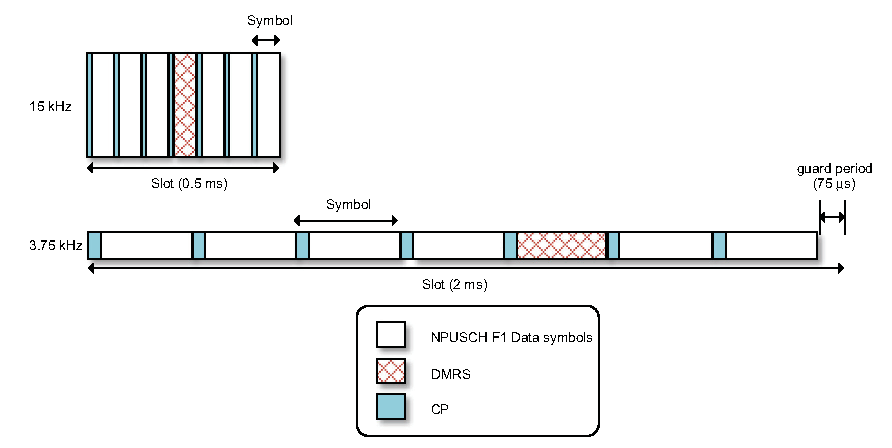
\includegraphics[width=\textwidth]{figures/NPUSCH1_structure.pdf}
\caption{The structure of NPUSCH format 1 \citep{NB-IoT_Book}}
\label{fig:NPUSCH1_structure}
\end{figure}
\end{minipage}%
\hfill
\begin{minipage}{0.48\textwidth}
\begin{figure}[H]
\centering
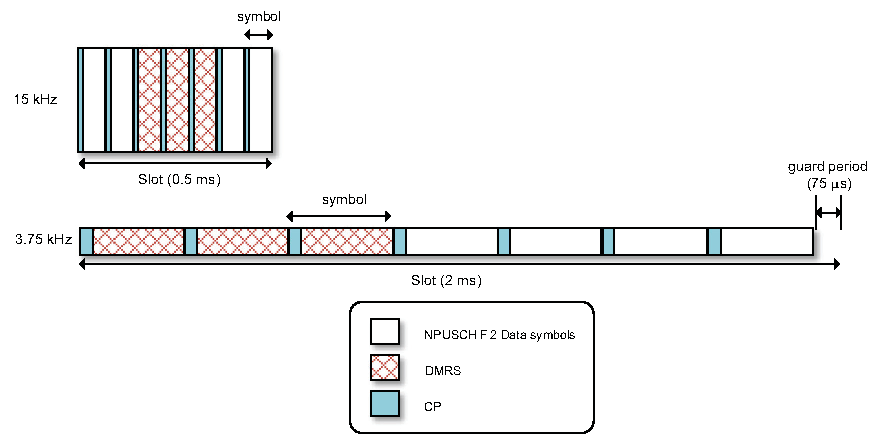
\includegraphics[width=\textwidth]{figures/NPUSCH2_structure.pdf}
\caption{The structure of NPUSCH format 2 \citep{NB-IoT_Book}}
\label{fig:NPUSCH2_structure}
\end{figure}
\end{minipage}


\begin{figure}[H]
\centering
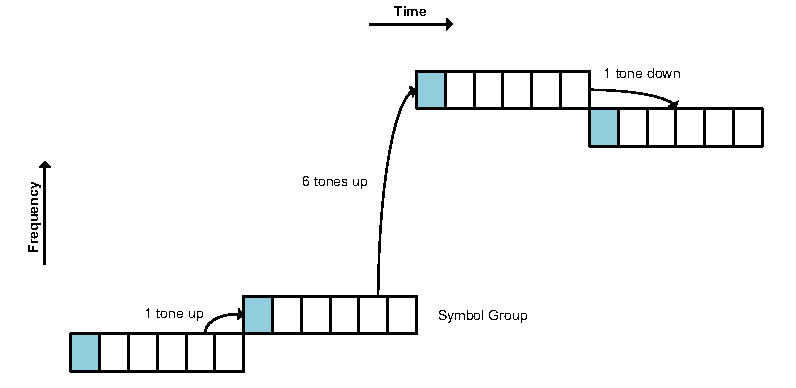
\includegraphics[width=0.5\textwidth]{figures/NPRACH_frequency_hopping.pdf}
\caption{The structure of a NPRACH symbol group \citep{NB-IoT_Book}}
\label{fig:NPRACH_structure}
\end{figure}

Channels\\
The \gls{UL} consists of two channels and one signal, namely the \gls{NPRACH}, \gls{NPUSCH} and \gls{DMRS}.

The \gls{NPRACH} consist of a repetition of four symbol groups, for each symbol group \gls{CP} is attached followed by five symbols. The duration of the CP is dependent CP-format chosen this can be seen in \autoref{fig:NPRACH_structure}, and depending on the coverage level the \gls{NPRACH} might be repeated up to 128 times. \citep{NB-IoT_Book}

The \gls{NPUSCH} carries the data transmission form the device and \gls{HARQ} acknowledgement for \gls{NPDSCH}. This is referred to as format 1 and 2 respectively, format 1 can carry up 1000 bits per transport block. As seen on \autoref{fig:NPUSCH1_structure} and \autoref{fig:NPUSCH2_structure} the DMRS, which is used for channel estimation at the base station, is multiplexed with the NPUSCH. 



